\documentclass[../notes.tex]{subfiles}

\graphicspath{{\subfix{../img/}}}

\begin{document}

\part{ECE349: Introduction to Energy Systems}


\marginnote{Taught by Prof. P. Lehn}
\section{Admin stuff}
\subsection{Lecture 1}
First lecture was logistical info + a speil about how power systems are one of the great modern wonders. Course will cover sinusoidal AC power systems (1, 3 phase), power systems (dc-dc, dc-ac conversion), and magnetic systems (transformers, actuators, and synchronous machines)

\subsubsection{Mark breakdown}

\begin{itemize}
	\item 50 \% Final
	\item 25 \% Midterm
	\item 5 \% Quiz
	\item 15 \% Labs
	\item 5 \% Assignments
\end{itemize}



\section{AC Steady State Analysis}
\subsection{Lecture 2}
\marginnote{
	Recall, for a general phasor $ \hat{P} $ 

	\begin{itemize}
		\item $ \frac{d \hat{P}}{dt} = jw \hat{P} $ 
		\item $ \int \hat{P} = \frac{1}{jw} \hat{P} $
	\end{itemize}
}

\subsubsection{TODO}
\begin{itemize}
	\item Review Thomas 669-600
\end{itemize}

What we have learnt prior for differential equations enables us to arrive at analytical solutions to linear stable AC systems with phasors.
A homogeneous and particular solution will be produced.
If there's a stable homogeneous solution, $ \to 0 $ as $ t \to \infty $. The full solution would be the addition of the two via super position.

We generally use this approach to solve circuits since it's an efficient way to solve circuits and make them into essentially DC circuits.

\begin{figure}[H]
	\centering
	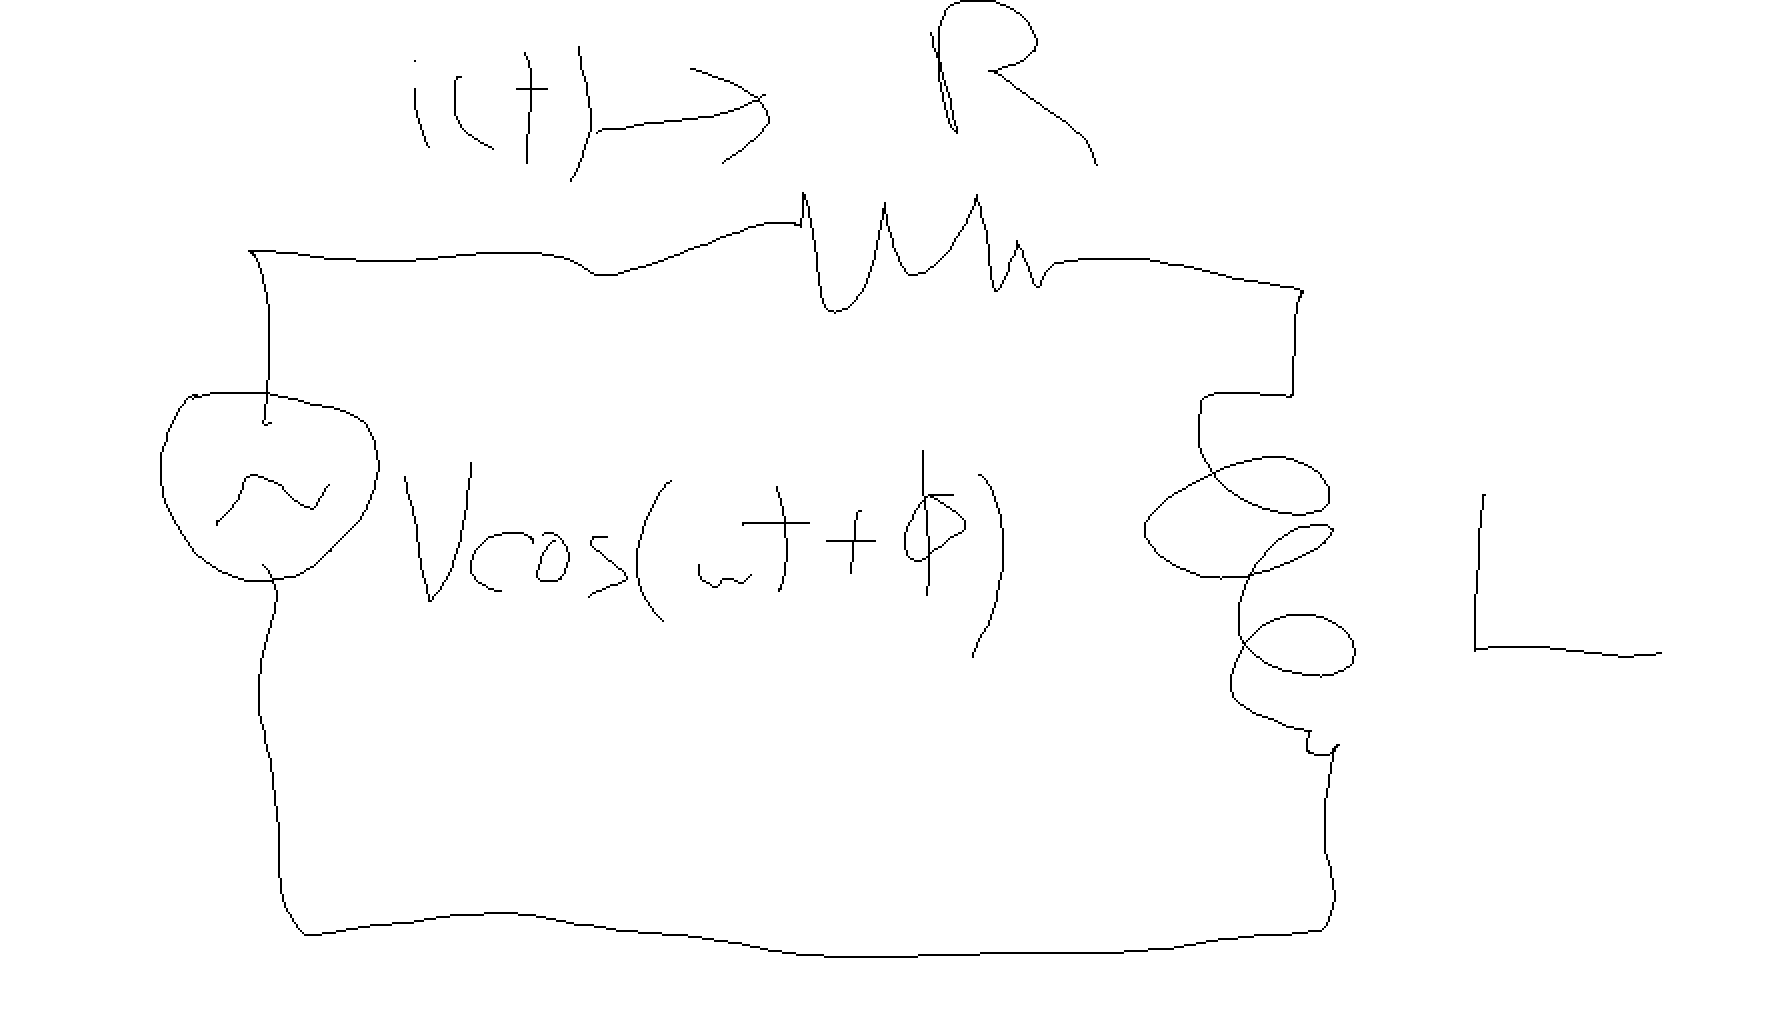
\includegraphics[width=0.8\linewidth]{img/image_2022-09-09-15-23-06.png}
\end{figure}

\begin{equation}
	\begin{split}
		Ri + L \frac{di}{dt} &= V \cos{(\omega t + \phi)}  \\
	\end{split}
\end{equation}


But this is a pain to solve. It can be made simpler by applying phasors

\begin{equation}
	V \cos{(\omega t + \phi)}  = Re\{ Ve^{j(\omega t + \phi)} \}
\end{equation}

Take the real part of $ \hat{I} $:

\begin{equation}
	R \hat{I} + L \frac{d\hat{I}}{dt} = Ve^{j(\omega t + \phi)}
\end{equation}


And therefore by inspection the solution is of format $ \hat{I} e^{j\omega t} $, where $ \hat{I} $ is a phasor. Noting that $ \hat{I} $  contains only amplitude and phase,

\begin{equation}
	\begin{split}
	R \hat{I} e ^{j \omega t} + L \frac{d}{dt}(\hat{I} e^{j \omega t}) &= Ve^{j \omega + \phi} \\
		R \hat{I} + L \hat{I} j \omega  &= Ve^{j \phi} \\
\end{split}
\end{equation}

And now reconstructing:

\begin{equation}
	\begin{split}
		\hat{I} &= \frac{V}{\sqrt{R^2 (\omega L)^2}} e^{j(\omega t + \phi - \tan^{-1}{\frac{wL}{R}})} \\
		 i(t) &= Re \left\{ \hat{I} \right\}   \\
	\end{split}
\end{equation}

And therefore

\begin{equation}
	\hat{I} = \frac{V}{\sqrt{R^2 (\omega L)^2}} \cos{(\omega t + \phi - \tan^{-1}(\frac{wL}{R}))}
\end{equation}


The steps to solving a phasor problem are:\marginnote{Notation: $ Xe^{j\phi} \leftrightarrow X\lfloor\phi $ }
\begin{itemize}
	\item Define phasor: $ V \cos{(\omega t + \phi)} \leftrightarrow V\lfloor\phi $ 
	\item Map $ L, C $ into phasor domain; find impedences
		\begin{itemize}
			\item $ v = L \frac{di}{dt} \leftrightarrow \hat{V} = j \omega L \hat{I} $ 
			\item $ i = C \frac{dv}{dt} \leftrightarrow \hat{V} = \frac{1}{j \omega C }\hat{I} $ 
		\end{itemize}
	\item Do mesh analysis to find $ \hat{I} $; $ \hat{I} = \frac{\hat{V}}{\sum \text{impedances} } $ 
	\item Reconstruct $ i(t) $ from $ \hat{I} $ 
\end{itemize}


\subsection{Lecture 3}

Phasors allow us to solve circuits with multiple sources of differing frequencies.



\begin{figure}[H]
	\centering
	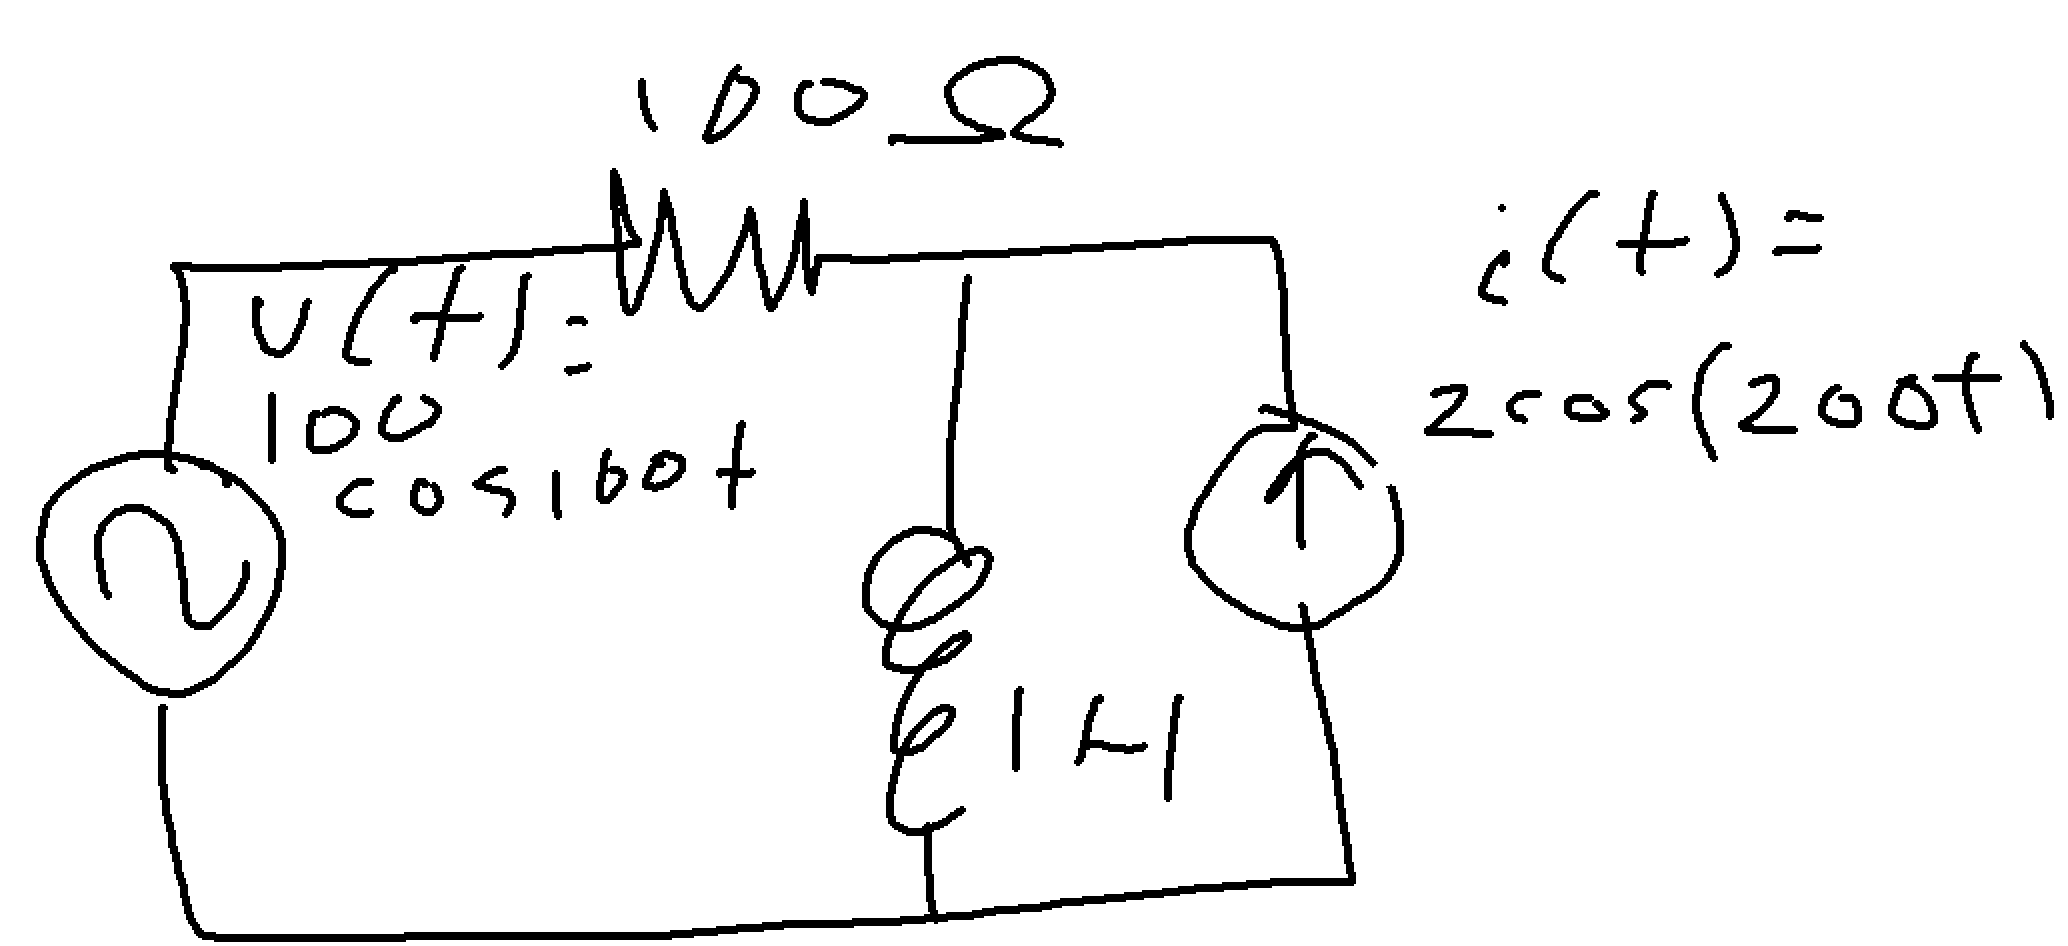
\includegraphics[width=0.8\linewidth]{img/image_2022-09-12-11-19-00.png}
\end{figure}

To find the current $ i(t) $ over the inductor we can find it's response due to the voltage and current sources and then apply superposition.

\begin{itemize}
	\item $ I_1 = \frac{100\lfloor{0}}{1oo + j100} = 0.707\lfloor{-45^o} \rightarrow i_1(t) = 0.707 cos(100t - 45^o) $ 
	\item $ I_2 = \frac{100}{100 + j200} 2\lfloor 0 = 0.894 \lfloor -65^o \rightarrow i_2(t) = 0.894 cos (200t - 63^o)$ 
	\item $ i(t) = i_1(t) + i_2(t) = 0.707cos(100t - 45^o) + 0.894 cos(200t - 63^o) $ 
\end{itemize}

Non-sinusoidal stimulus may be solved by decomposing the signal with Fourier transforms. 
For example, square waves:

\begin{figure}[H]
	\centering
	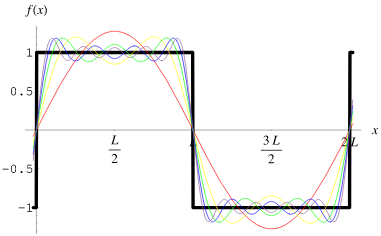
\includegraphics[width=0.8\linewidth]{img/image_2022-09-12-11-28-11.png}
	\caption{square waves with Fourier series superimposed}
\end{figure}

The general form of a Fourier transform is given as:

\begin{equation}
	v_{equiv}(t) = a_o + \sum^\infty_{n=1} a_k cos(nw_ot) + b_k cos(nw_ot)
	\label{eq:349:fourier}
\end{equation}

Where:

\begin{equation}
	\begin{split}
		a_o &=  \frac{1}{T} \int^T_0 v(t) dt \\
		a_k &= \frac{2}{T} \int^T_0 v(t) cos (nw_o t) dt \\
		b_k &= \frac{2}{T} \int^T_0 v(t) sin(nw_o t) dt \\
	\end{split}
	\label{eq:349:fourier_terms}
\end{equation}


Armed with Fourier series and superposition we may now model a non-sinusoidal signal as a superposition of an infinite sum of sources. About half the work can be cut in half by recognizing that $ sin $ lags $ cos $ by $ 90^o $, so


\begin{equation}
	\begin{split}
		a_o &=  \frac{1}{T} \int^T_0 v(t) dt \\
		a_k &= \frac{2}{T} \int^T_0 v(t) cos (nw_o t) dt \\
		b_k &= \frac{2}{T} \int^T_0 v(t) cos(nw_o t - 90^o) dt \\
	\end{split}
\end{equation}

\section{AC Power}

\begin{definition}
	\textbf{Instantaneous Power}: $ p(t) = v(t) \times i(t) [W, \frac{J}{s}]$  

	\begin{example}
		For a circuit with a voltage source, $ v(t) = Vcos(\omega t) $ and a resistor $ \Omega $, $ i(t) = Icos(\omega t) $, $ p(t) = VI cos^2 (\omega t) = \frac{VI}{2}(1+cos(2\omega t))$
	\end{example}
	
\end{definition}

\begin{definition}
	\textbf{Average Power over Cycle}: $ P(t) = \frac{1}{T} \int_o^T p(t) dt = \frac{VI}{2} $  
\end{definition}

If we were to plot the instantaneous power we see that due to the sinusoidal response there are times where $ 0 $ power is supplied.
This will always be true for a single phase power supply; real-world supplies always have multiple phases; this is why computer PSUs always contain a ton of capacitors.


\begin{definition}
	\textbf{Reactive Power}: $ Q $ 


	\begin{figure}[H]
		\centering
		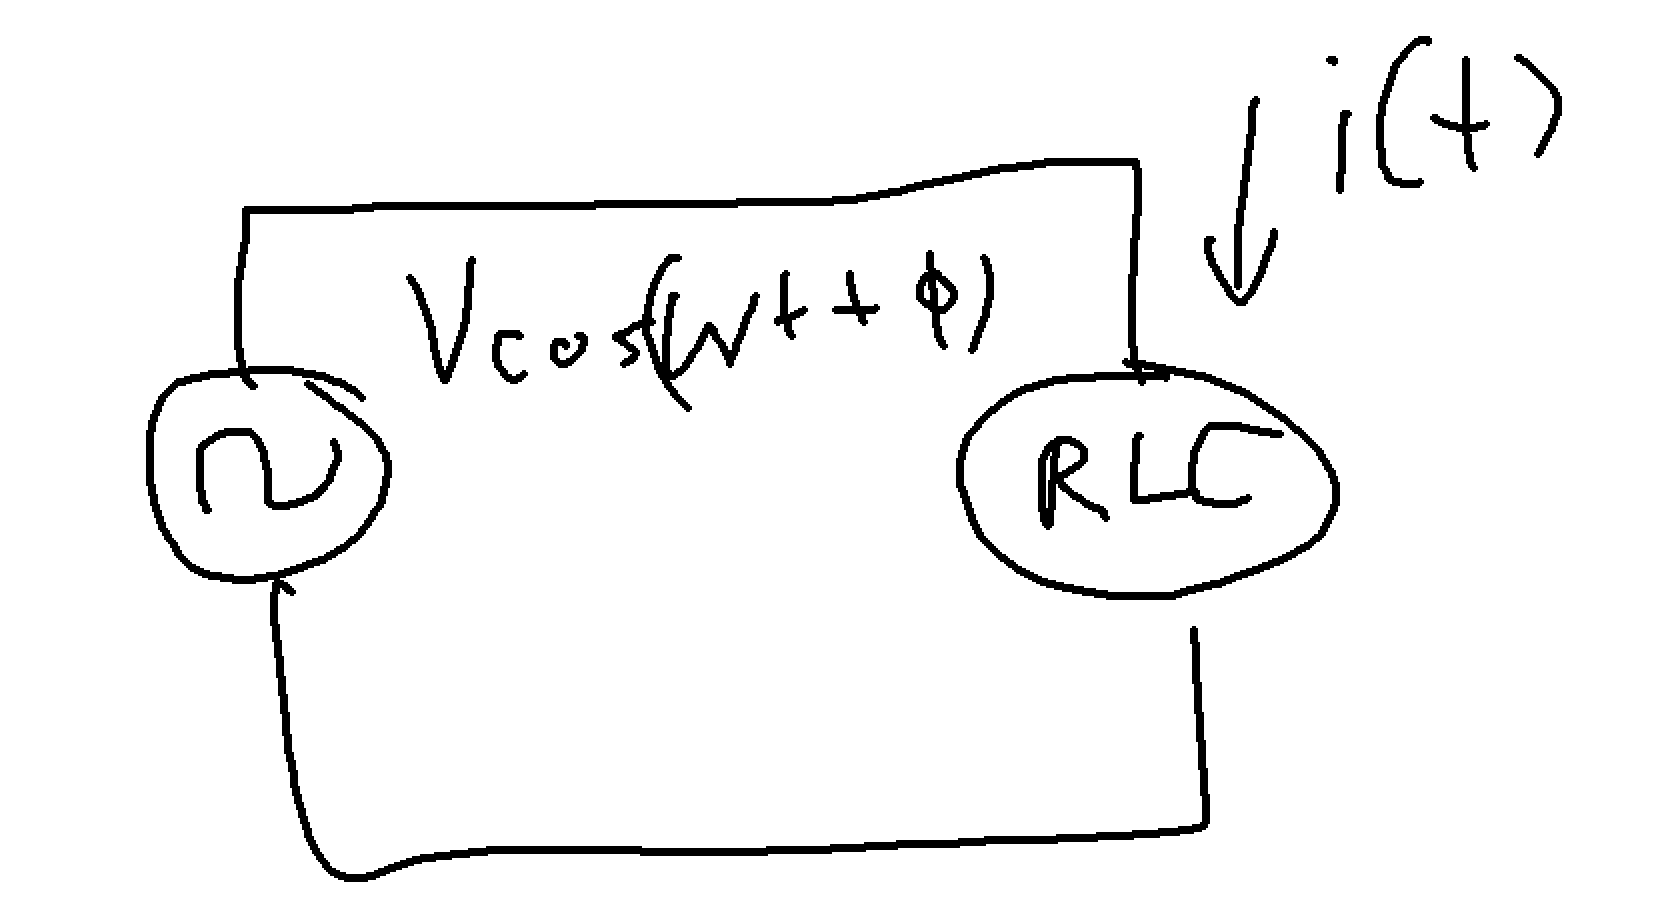
\includegraphics[width=0.8\linewidth]{img/image_2022-09-12-11-49-46.png}
	\end{figure}

	\marginnote{$ \phi = \phi_v - \phi_i $ }

	If $ \phi_i = 0$ and taking $ \phi = \phi_v $,

	\begin{equation}
		\begin{split}
			p(t) &= V\cos(\omega t + \phi) * I \cos(\omega t) \\
					 &= \frac{VI}{2} \cos(\phi) + \cos(2\omega t + \phi) \\
					 &= \underbrace{\frac{VI}{2} \cos(\phi)(1 + \cos(2 \omega t)}_{\text{real power e.g. heat}} 
					 - \underbrace{\frac{VI}{2} (\sin \phi \sin 2 \omega t)}_{\text{stored and released back to source}} \\
		\end{split}
	\end{equation}

	Taking the average power of the reactive power we get 

	\begin{equation}
		P_{avg} = \frac{VI}{2} \cos\phi
	\end{equation}
	Another quantity, reactive power, can be defined with regards to the energy sloshing back and forth:

	\begin{equation}
		Q = \frac{VI}{2} \sin \phi
		\label{eq:349:reactive_power_q}
	\end{equation}
	

\end{definition}

\subsection{Lecture 4}


\begin{definition}
	\textbf{Displacement factor} 

	$ DF \equiv \cos \phi $ 

	Where $ \phi $ is the angle measured from the $ \hat{V} $ to the $ \hat{I} $ phasors.
	A $ DF = 1 $ means the system is transferring the most power possible.

	\begin{itemize}
		\item Lagging DF: $ \phi  $ is -'ve
		\item Leading DF: $ \phi  $ is +'ve'
	\end{itemize}
\end{definition}


We can also write $ P, Q$ from phasors.

\begin{equation}
	\begin{split}
		P  &= \frac{\hat{V} \hat{I}}{2} \cos(\phi_v - \phi_i) \\
			 &= \frac{1}{2} \hat{V} \hat{I} Re\{e^{j\phi_v - \phi_i}\} \\
			 &= \frac{1}{2} Re\{Ve^{j\phi v} \cdot I e^{-j\phi_i}  \} \\
			 &= \frac{1}{2} Re\{\hat{V} \hat{I^*}\} \\
	\end{split}
\end{equation}

\begin{equation}
	\begin{split}
		Q  &= \frac{\hat{V} \hat{I}}{2} \sin(\phi_v - \phi_i) \\
		\vdots \\
			 &= \frac{1}{2} Im \{\hat{V} \hat{I^*}\} \\
	\end{split}
\end{equation}


The expressions for $ Q $  and $ P $ are basically the same so we define a new quantity, complex power, which incorporates both the imaginary and real components.

\marginnote{Reference: Thomas 16.1, 16.2, 16.3}

\begin{definition}
	\textbf{Complex Power} 
	\begin{equation}
		S = \frac{1}{2} \hat{V} \hat{I*} = P + jQ
		\label{eq:349:complex_power}
	\end{equation}
	
\end{definition}


\subsubsection{Root Mean Squared (RMS) Values}


A RMS value measures the average power of a periodic signal. Consider a circuit with an AC voltage source with $ v(t) $ flowing through a resistor. 


The power is:
\begin{equation}
	p(t) = v(t) i(t) = v(t) \frac{v(t)}{R} = \frac{1}{R} v(t)^2
\end{equation}

The average power is therefore

\begin{equation}
	P = \frac{1}{R} \int_0^T v(t)^2 dt
\end{equation}


Evaluating this becomes easier by defining an useful quantity, RMS voltage

\begin{equation}
	v_{rms} = \sqrt{\frac{1}{T} \int^T_0 v(t)^2 dt} 
\end{equation}
	

And using $ v_{rms} $ we get a nice expression for average power,

\begin{equation}
	P = \frac{1}{R} v_{rms}^2
\end{equation}



More generally speaking we can define RMS values of sinusoidal signals

\begin{definition}
	\begin{equation}
		v_{rms} = \sqrt{\frac{1}{2\pi} \int^{2\pi}_0 (\hat{V} \cos wt )^2 dt}  = \frac{1}{\sqrt{2}}  \hat{V}
	\end{equation}
\end{definition}


Plugging this into the expressions for complex power:

\begin{equation}
	S = \underline{V} \cdot \underline{I^*}
\end{equation}

Where $ \underline{V} $, $ \underline{I^*} $ are RMS phasors at a given common frequency.


And more generally yet, the RMS values of non-sinusoidal signals can be found with help of a Fourier expansion


\begin{definition}
	Let $ v(t) = \hat{v}_0 + \hat{v}_1 \cos(wt+\phi_1) + \ldots $ 

	Then,


	\begin{equation}
		v_{rms} = \sqrt{\hat{v}^2 + \frac{\hat{v}_1}{\sqrt{2} }^2 + \frac{\hat{v}_2}{\sqrt{2} }^2 \ldots }   = \sqrt{v_0^2 + \sum^\infty_{n=1} (\frac{V_m^2}{2})} 
	\end{equation}

	And if $ V_m $ is the $ rms $ value,

	\begin{equation}
		v_{rms} = \sqrt{v_0^2 + \sum^\infty_{n=1} V_m^2} 
	\end{equation}
	

\end{definition}

One thing to watch out for is that we could have a system with high voltage but near-zero current transferring little to no power. 
To account for this we look at the power factor `PF'

\begin{definition}
	\textbf{Power Factor} 
	\begin{equation}
		PF \equiv \frac{\text{average power}}{\text{rms voltage} \cdot  \text{rms current}}
	\end{equation}
\end{definition}

For a sinusoidal $ V, I $:


\begin{equation}
	\begin{split}
		PF &= \frac{\frac{1}{2} \hat{V} \hat{I} \cos \phi}{  \frac{\hat{V}}{\sqrt{2} } \cdot  \frac{\hat{I}}{\sqrt{2} }  }  \\
		 &=  \cos\phi\\
	\end{split}
\end{equation}


If signals are not harmonics $ PF = DF $. This can be a source of confusion. 


For non-sinusoidal systems this becomes more difficult because, unlike pure signals, they may contain harmonics.
In these systems either $ V, I $, or both may contain harmonics. 
Generally in household power $ V $ is clean but $ I $ contains harmonics.


The effect of harmonics in currents is that $ I_{\text{harmonics}} $ causes a higher $ I_{rms} $; there is more current but no higher power!
This reduces $ PF $ and causes $ PF < DF $.


To summarize, 

\begin{itemize}
	\item In ideal systems, $ PF = DF $ if all $ V $ and $ I $ are at one frequency.
	\item $ PF = 1 $ means no energy sloshing between load and source.
\end{itemize}

Harmonics are bad because they reduce the usefulness of the system
There are very tight standards for how many harmonics one is allowed to inject into the system via generators or loads.
See: textbook 16.6




\subsection{Lecture 5: Multi-Phase AC}


AC power is generated by spinning a magnet between some coils.
Some pixies get excited and by some Maxwell's equations and EMF and ECE259 we get a voltage induced in the coils.

\begin{figure}[H]
	\centering
	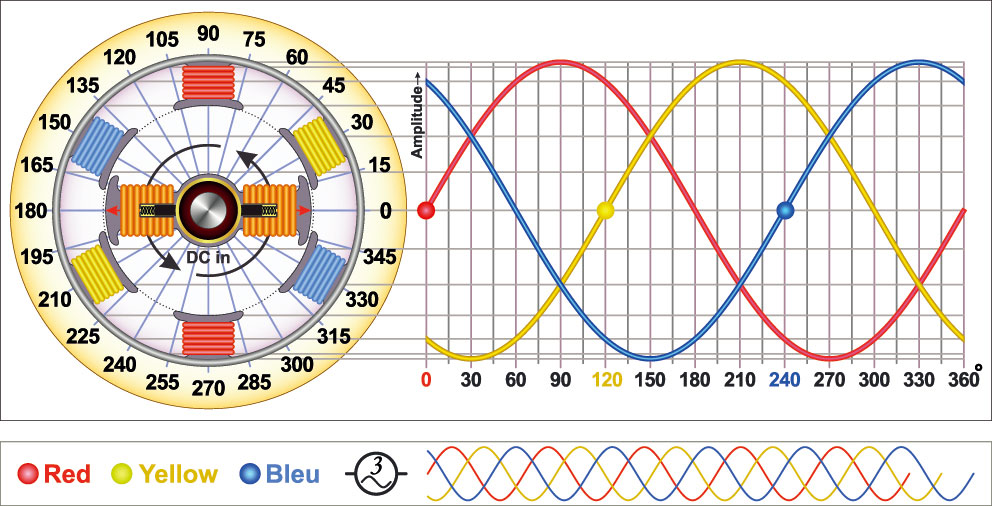
\includegraphics[width=0.8\linewidth]{img/image_2022-09-17-21-36-37.png}
\end{figure}

Current from a generator with a single pair of coils is \textit{single phase}.
Most generators, like the one in the picture, have three pairs of coils and therefore generate three phases.
For a typical three-phase setup with coils arranged at $ 0^o, 120^o, 240^o $, the voltages can be found with a little bit of trigonometry.


\begin{equation}
	\begin{split}
		v_{a}(t) &= \sqrt{2} V \cos \omega t  \rightarrow \underline{V_{a}} = V \lfloor 0  \\
		v_{b}(t) &= \sqrt{2} V \cos( \omega t - 120) \rightarrow  \underline{V_{b}} = V \lfloor -120^o\\
		v_{c}(t) &= \sqrt{2} V \cos (\omega t - 240) \rightarrow \underline{V_{c}} = V \lfloor 240^o\\
	\end{split}
\end{equation}


And similar expressions may be derived for single-phase and two-phase power.


The reason why three-phase power is typically used has to do with efficiency of power transfer relative to the amount of wires and copper needed.
Whereas single-phase power requires two wires to carry power and two-phase power requires four wires, three-phase power can be transmitted over 6, 4, or three wires.
This saves a lot of copper as three-phase $ 3\phi $ power can carry 50\% more power than $ 2\phi $ power for less copper.



In $ 3\phi $ systems the voltages sum to zero; $ v_a(t) + v_b(t) + v_c(t) = 0 \forall t$ 

Four-wire three-phase power:


\begin{figure}[H]
	\centering
	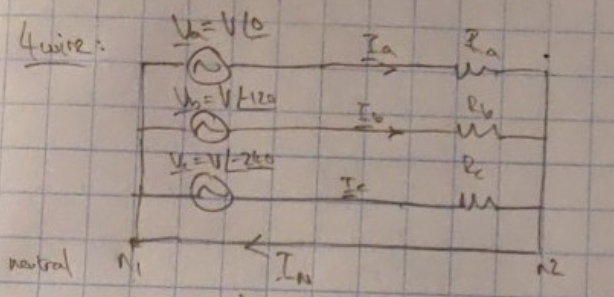
\includegraphics[width=0.8\linewidth]{img/image_2022-09-18-02-19-51.png}
	\caption{A four wire system for three phase power}
\end{figure}

If $ R_a = R_b = R_c = R $, we have a balanced load and then the currents are related by $ i_n = i_a(t) + i_b(t) + i_c(t) = 0 $.
\marginnote{Proof: just substitute the condition earlier that voltages sum to zero and the fact that all resistances are equal into $ I = \frac{V}{R} $ }


Three-wire systems drop the fourth neutral wire since it carries no current. This can be problematic if the load is not balanced; though $ I_a + I_b + I_c = 0$  will still hold true since there is no return path, the nodes at either end of the AC source and resistor pair would have differing voltages.


If the system is balanced then to save ourselves from drawing everything out all the time, only a single diagram is drawn for a characteristic phase and then solved once.


\begin{example}
	\begin{equation}
		Z_a = Z_b = Z_c = Z
	\end{equation}
	\begin{equation}
		\underline{V_b}
		\underline{V_a} e^{\frac{-j_2n}{3}}
	\end{equation}

	\begin{equation}
		\underline{V_c}
		\underline{V_a} e^{\frac{-j_4n}{3}}
	\end{equation}

	Then,

	\begin{equation}
		\underline{I_a} = \frac{\underline{V_a}}{Z}
	\end{equation}
	\begin{equation}
		\underline{I_b} = \frac{\underline{V_b}}{Z} = \frac{\underline{V_a}}{Z} e^{\frac{-j_2n}{3}}
	\end{equation}

	\begin{equation}
		\underline{I_b} = \frac{\underline{V_c}}{Z} = \frac{\underline{V_a}}{Z} e^{\frac{-j_4n}{3}}
	\end{equation}

	And then the solutions for phase b and c are the same as that for phase a except for the $ 120^o, 240^o$  offsets.
	
\end{example}


Because of this property, instead of drawing three separate diagrams for each phase, we can just draw one diagram and then solve for the other two phases.
\begin{figure}[H]
	\centering
	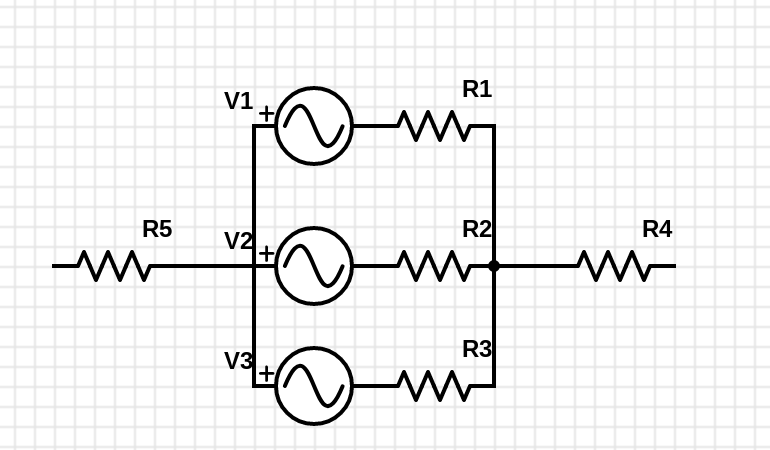
\includegraphics[width=0.8\linewidth]{img/image_2022-09-18-02-32-50.png}
\end{figure}

\begin{figure}[H]
	\centering
	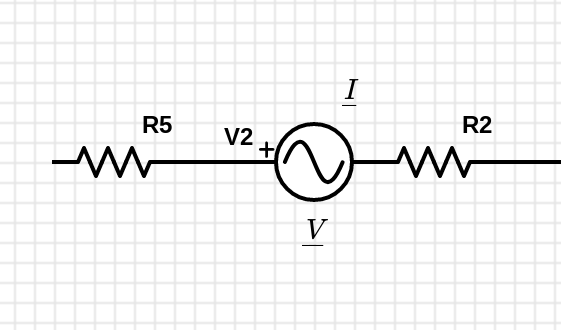
\includegraphics[width=0.8\linewidth]{img/image_2022-09-18-02-35-24.png}
	\caption{Condensed diagram for three phase power}
\end{figure}


\subsection{Lecture 6: Y and Delta connections }

\begin{figure}[H]
	\centering
	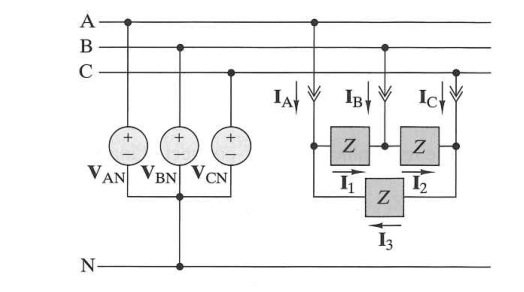
\includegraphics[width=0.8\linewidth]{img/image_2022-09-19-11-25-58.png}
	\caption{Three-phase system with a $ Y $ connected source and a $ \Delta $ connected load}
\end{figure}

The current to ground $ I_N $ is always $ 0 $ for a $ \Delta $ connected load. $ I_N $ is zero for a $ Y $ cnonnected load if $ Y $ has no neutral connection and the load/source are balanced.


\begin{theorem}
	\textbf{$ Y-\Delta $ conversion}

	Any $ \Delta $ load can be converted to a equivalent $ Y $ connected load

	\begin{figure}[H]
		\centering
		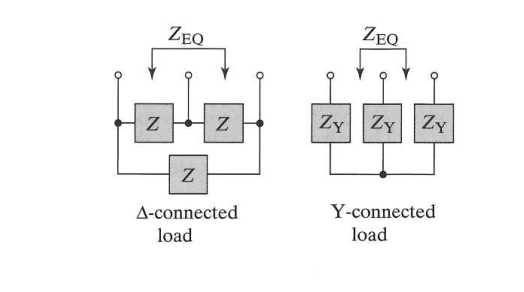
\includegraphics[width=0.8\linewidth]{img/image_2022-09-19-11-28-05.png}
	\end{figure}

\end{theorem}

The derivation is in the textbook.


Sources can be connected in $ Y $ or $ \Delta $ configurations.

\begin{definition}
	Line currents are the currents on the lines $ a, b, c $. Phase currents are the currents immediately beside the sources.
\end{definition}


\begin{figure}[H]
	\centering
	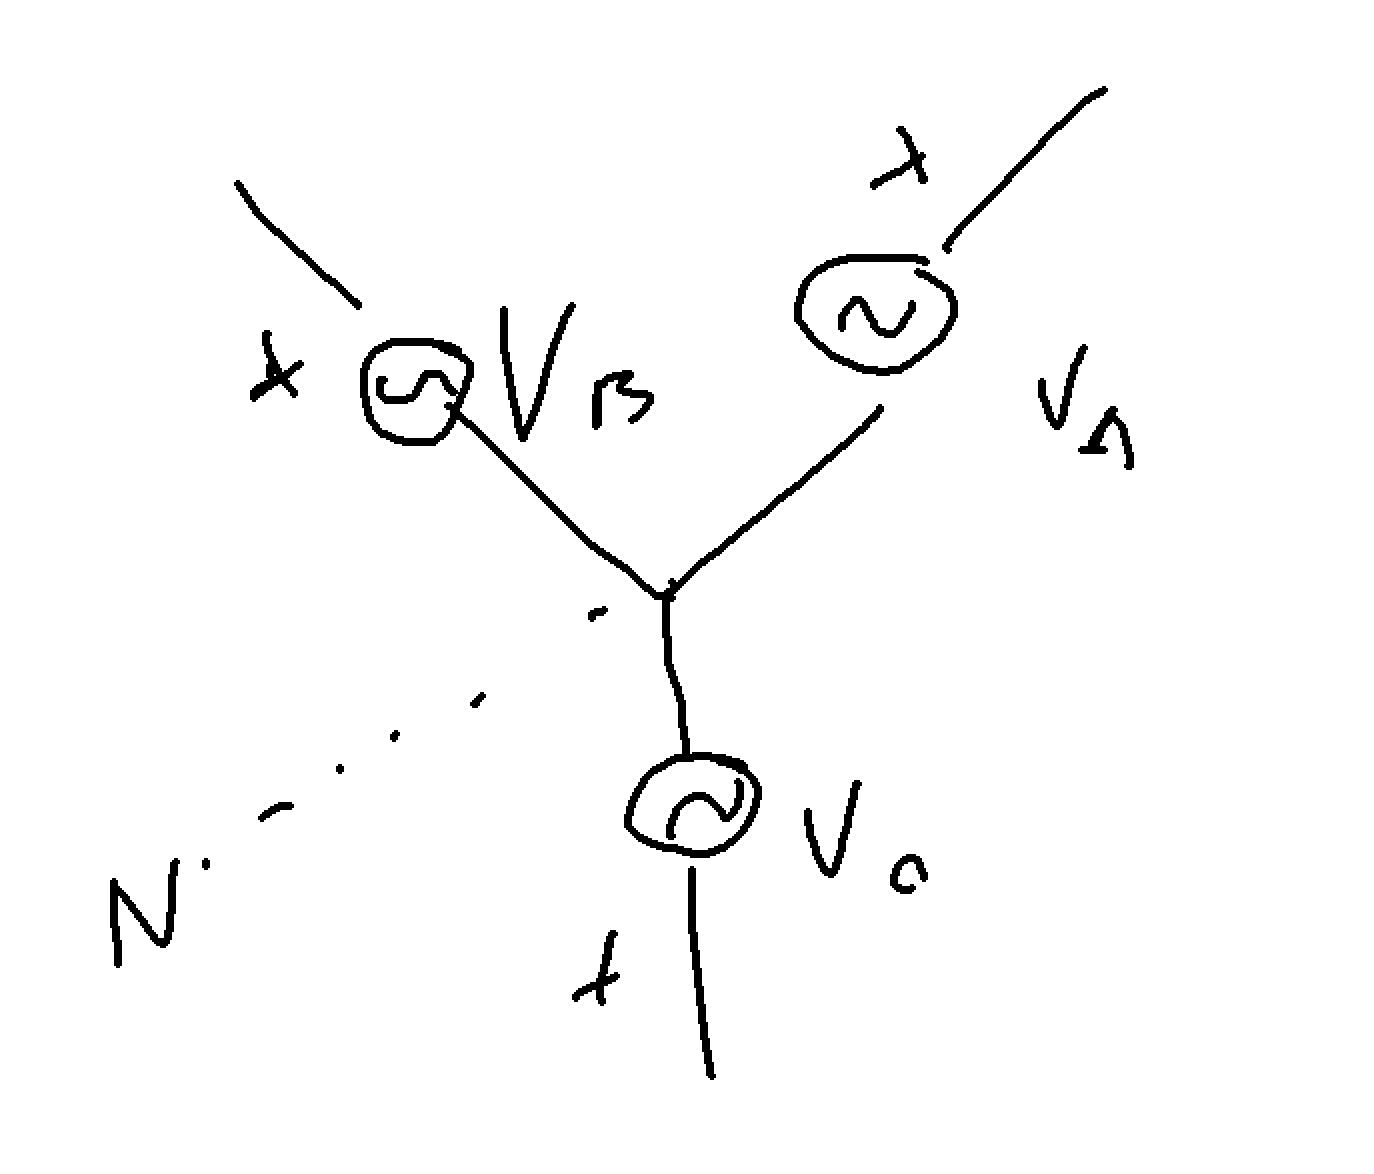
\includegraphics[width=0.8\linewidth]{img/image_2022-09-19-11-37-44.png}
\end{figure}

A $ Y $ connected source has the neutral line in the center.

\marginnote{Angle differences are $ 0, 120, 240 $ degrees }

\begin{equation}
	\tilde{V}_{AB} = \tilde{V}_A - \tilde{V}_B = |\tilde{V}_A| (1-1\lfloor e^{-\frac{2\pi}{3}}) = \sqrt{3}  |\tilde{V}_A| e^{ \frac{j\pi}{6}}
	\label{eq:349:y_source_volt}
\end{equation}

The line and phase current are the exact same in the case of a $ Y $ connected source.
However, the line and phase voltages are different and are related by~\eqref{eq:349:y_source_volt}.


\begin{figure}[H]
	\centering
	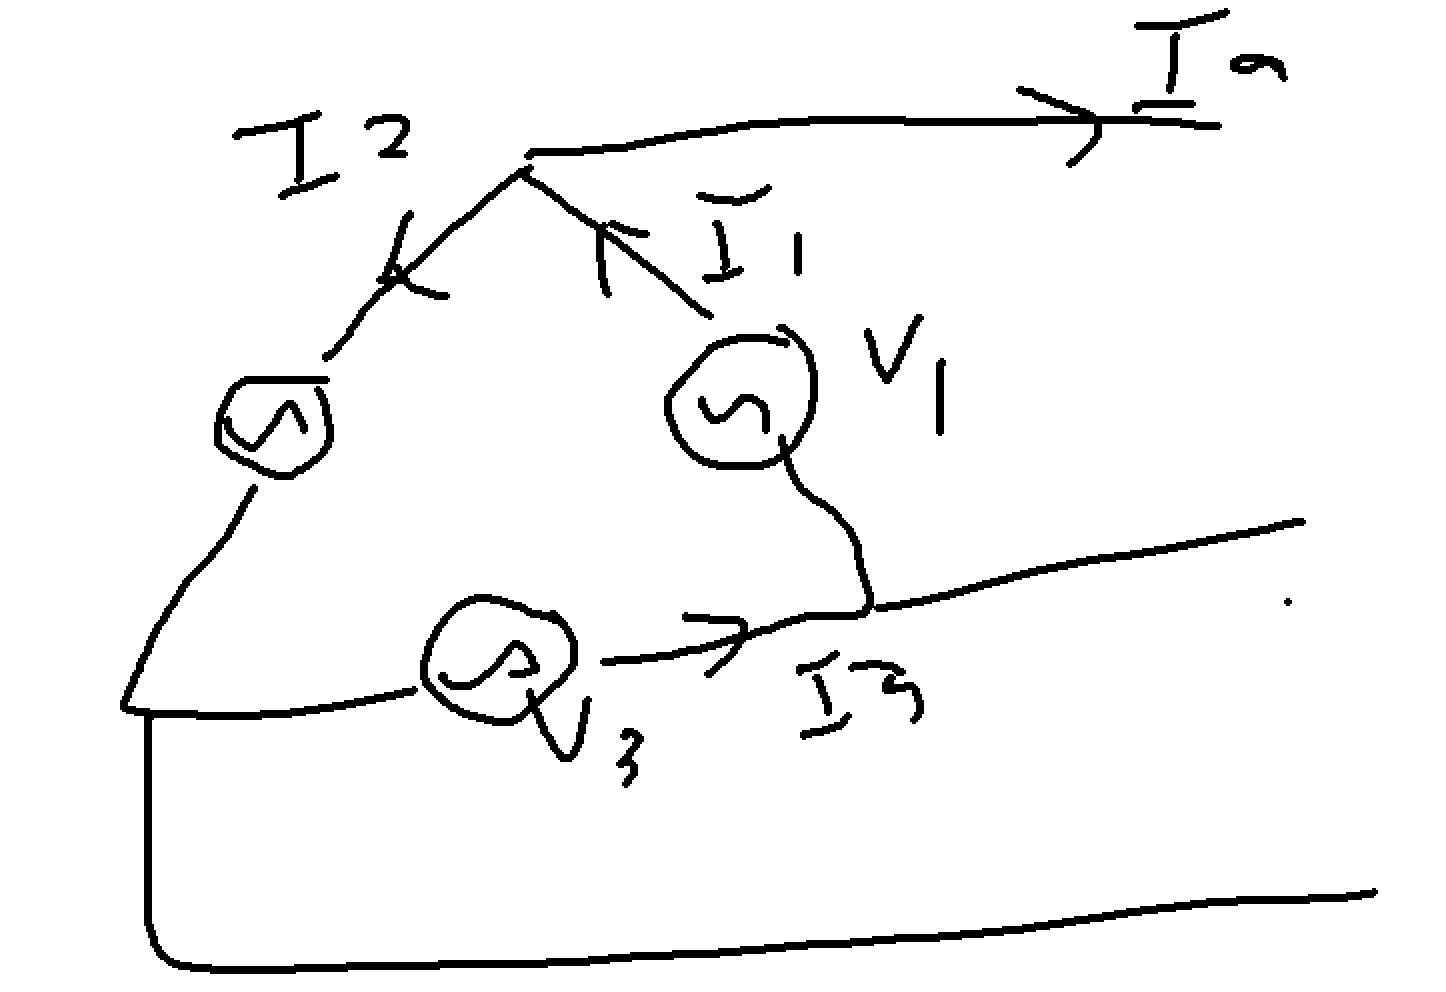
\includegraphics[width=0.8\linewidth]{img/image_2022-09-19-11-42-03.png}
\end{figure}


A $ \Delta $  connected source has no neutral point.

\begin{equation}
	I_a = I_1 - I_2 = I_1 (1- 1 \lfloor e^{-\frac{2\pi}{3}}) = \sqrt{3} I_1 e^{\frac{j\pi}{6}}
	\label{eq:349:delta_source_current}
\end{equation}

The line and phase voltages are the exact same in the case of a $ \Delta $ connected source.
However, the line current and phase currents are different and are related by~\eqref{eq:349:delta_source_current}.




Since neutral is not always available, we write $ 3\phi $ systems based on their line-to-line voltages.
For exampl,e, a $ 208V $ system has $ 120V_{rms} $ on each phase.


\begin{example}
	A $ Y $ connected three-phase source has a line-to-line voltage, i.e. $ V_{A \rightarrow B} $ of $ 208V$ but each source has $ 120V $ since $ \frac{208}{\sqrt{3} } = 120V $.
	A similar argument can be applied for the $ \Delta $ sources.

	\begin{equation}
		I = \frac{10}{\sqrt{3}  = 5.8A}
	\end{equation}
	
\end{example}



\subsection{Lecture 7: DC-DC conversion}

Let's say we want to supply $ 10V $  DC to a load but our supply is at 20.5V.
We have a few options. We can use a resistor to drop the voltage via a voltage divide, which we learned about in ECE159.
However this is not only not every efficient, but also non-responsive to changes in resistance load and will provide incorrect supply voltage if the load is not as anticipated.
Another option is to use \textbf{transistors} to regular the power instead.\marginnote{semiconductors to process power $ \Leftrightarrow $ power electronics }

\begin{figure}[H]
	\centering
	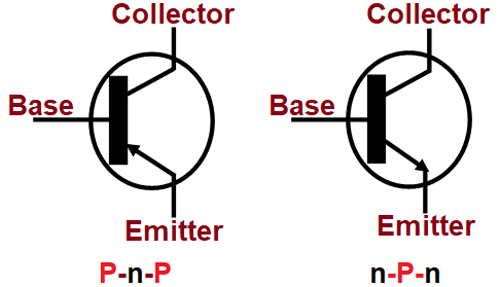
\includegraphics[width=0.8\linewidth]{img/image_2022-09-23-02-42-21.png}
	\caption{Transistors have a Base, Collector, and Emitter. At this point in the course, we just need to know that we can change the $ V-I $ response by fiddling with the base current $ i_B $   }
\end{figure}

\begin{figure}[H]
	\centering
	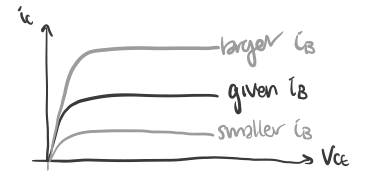
\includegraphics[width=0.8\linewidth]{img/image_2022-09-23-02-42-56.png}
	\caption{Thanks sherry for this figure}
\end{figure}


Finding the operating point that we want the transistor to be at can then be done graphically by solving a system of two equations with two unknowns, namely finding the intersection between the transistor response at at given $ i_B $ and the desired voltage/current of the load. 
Then the correct $ i_B $ can be selected.

However this is not very efficient since a lot of power is being wasted in the transistor. For a $ 20.5V $ source and a $ 10V $   load at $ 2A $, $ V_{CE} = 10.5V$ , so $ P_{loss} = 10.5 * 2 = 21W $  being lost in the transistor which results in the rather poor $ \frac{20}{20.5 * 2 = 41} \rightarrow \eta = 49\%$  efficiency.
So the transistor is a little bit better but we still lose half the power -- which means that in a device this would halve the battery life and require a huge heat sink. How can we do better?



\textbf{Switch-mode power} is a way to maximize $ \eta $  by switching between two states that correspond to low power loss at a high frequency

\begin{figure}[H]
	\centering
	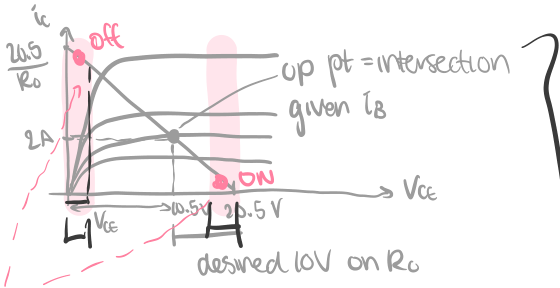
\includegraphics[width=0.8\linewidth]{img/image_2022-09-23-02-59-29.png}
\end{figure}

The left state is the `off' state and the right state is the `on' state. 
Switching rapidly between $ 20.5V, 0A $  and $ 0.5V, 4A$  results in what is, on which is on average what we want.
This will also produce the same power output while increasing efficiency


What about the timing between the off/on states? This can be found by taking an integral to find the relationship between $ T_{on} $  and $ T_{off} $  with respect to power.
\begin{equation}
	\begin{split}
		P &= \frac{1}{T} \int^T_0 p(t) dt\\
			&= \frac{1}{T} \int^{T_{on}}_0 i_c^2 R_o dt \\
			&= \frac{1}{T} \int^{T_{on}}_0 4^2 \cdot  5 dt \\
			&= 80 \frac{T_{on}}{T} \\
	\end{split}
\end{equation}

So in order to transfer the same $ 20W $  to the $ 5 \Omega $ load, we would use $ T_{on}/T = \frac{1}{4} $, which would correspond to $ P_{in} = V_{i} \cdot T_{on}/T = 20.5W  $. 
It then follows that $ \eta = \frac{20}{20.5} = 97.6\% $ which is much better\mn{compared to the $ 49\%  $ before }

A few points of caution:

\begin{itemize}
	\item A pulsing output voltage/power can be dangerous for some loads. For example motors aren't a fan of it. In these cases a filter can be applied to leave behind the average power.
	\item If we want to supply average voltage/power an on-time of $ 50\% $ would be required. 
\end{itemize}









\begin{figure}[H]
	\centering
	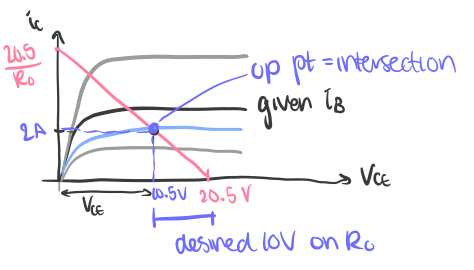
\includegraphics[width=0.8\linewidth]{img/image_2022-09-23-02-48-01.png}
\end{figure}




\subsection{Lecture 8: Average output voltage}


Consider a circuit with a transistor and a load.

\begin{figure}[H]
	\centering
	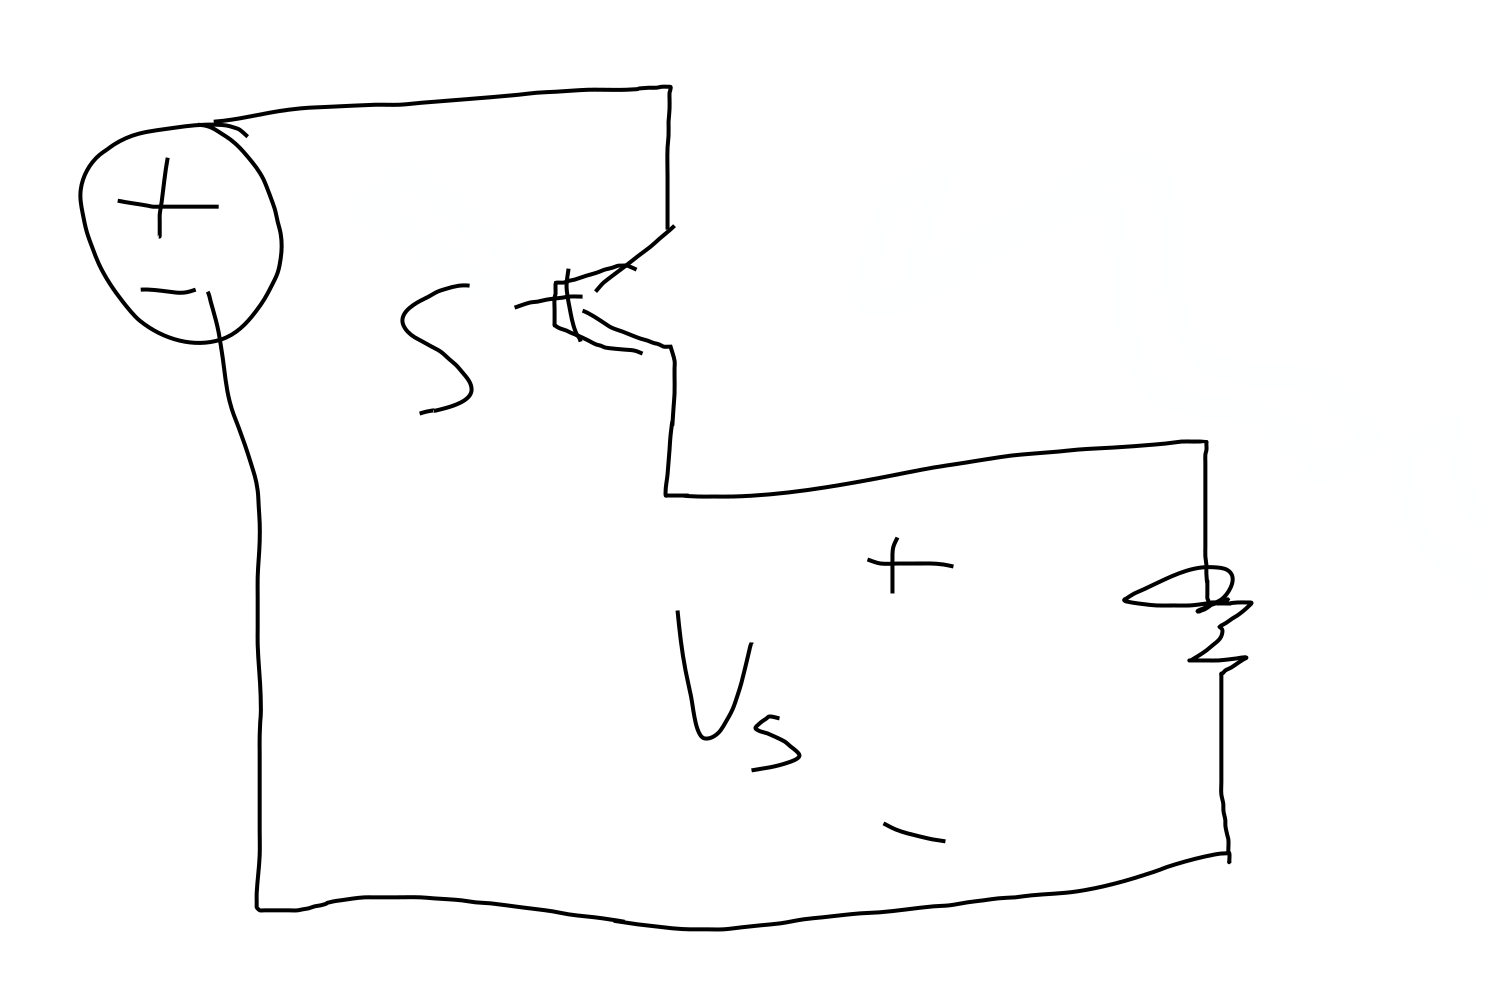
\includegraphics[width=0.8\linewidth]{img/image_2022-09-23-15-21-54.png}
\end{figure}



A switching signal $ S $ taking on a value from $ {0, 1} $  periodically over time is applied to the transistor

\begin{definition}
	\textbf{Duty cycle}: the fraction of time that $ S $ is $ 1 $

	\begin{equation}
		D = \frac{T_{on} }{T_s}
	\end{equation}
	
\end{definition}


The response of the circuit, where $ V_g $  is the source voltage and $ V_s $  being the voltage at the load would look like this:

\begin{figure}[H]
	\centering
	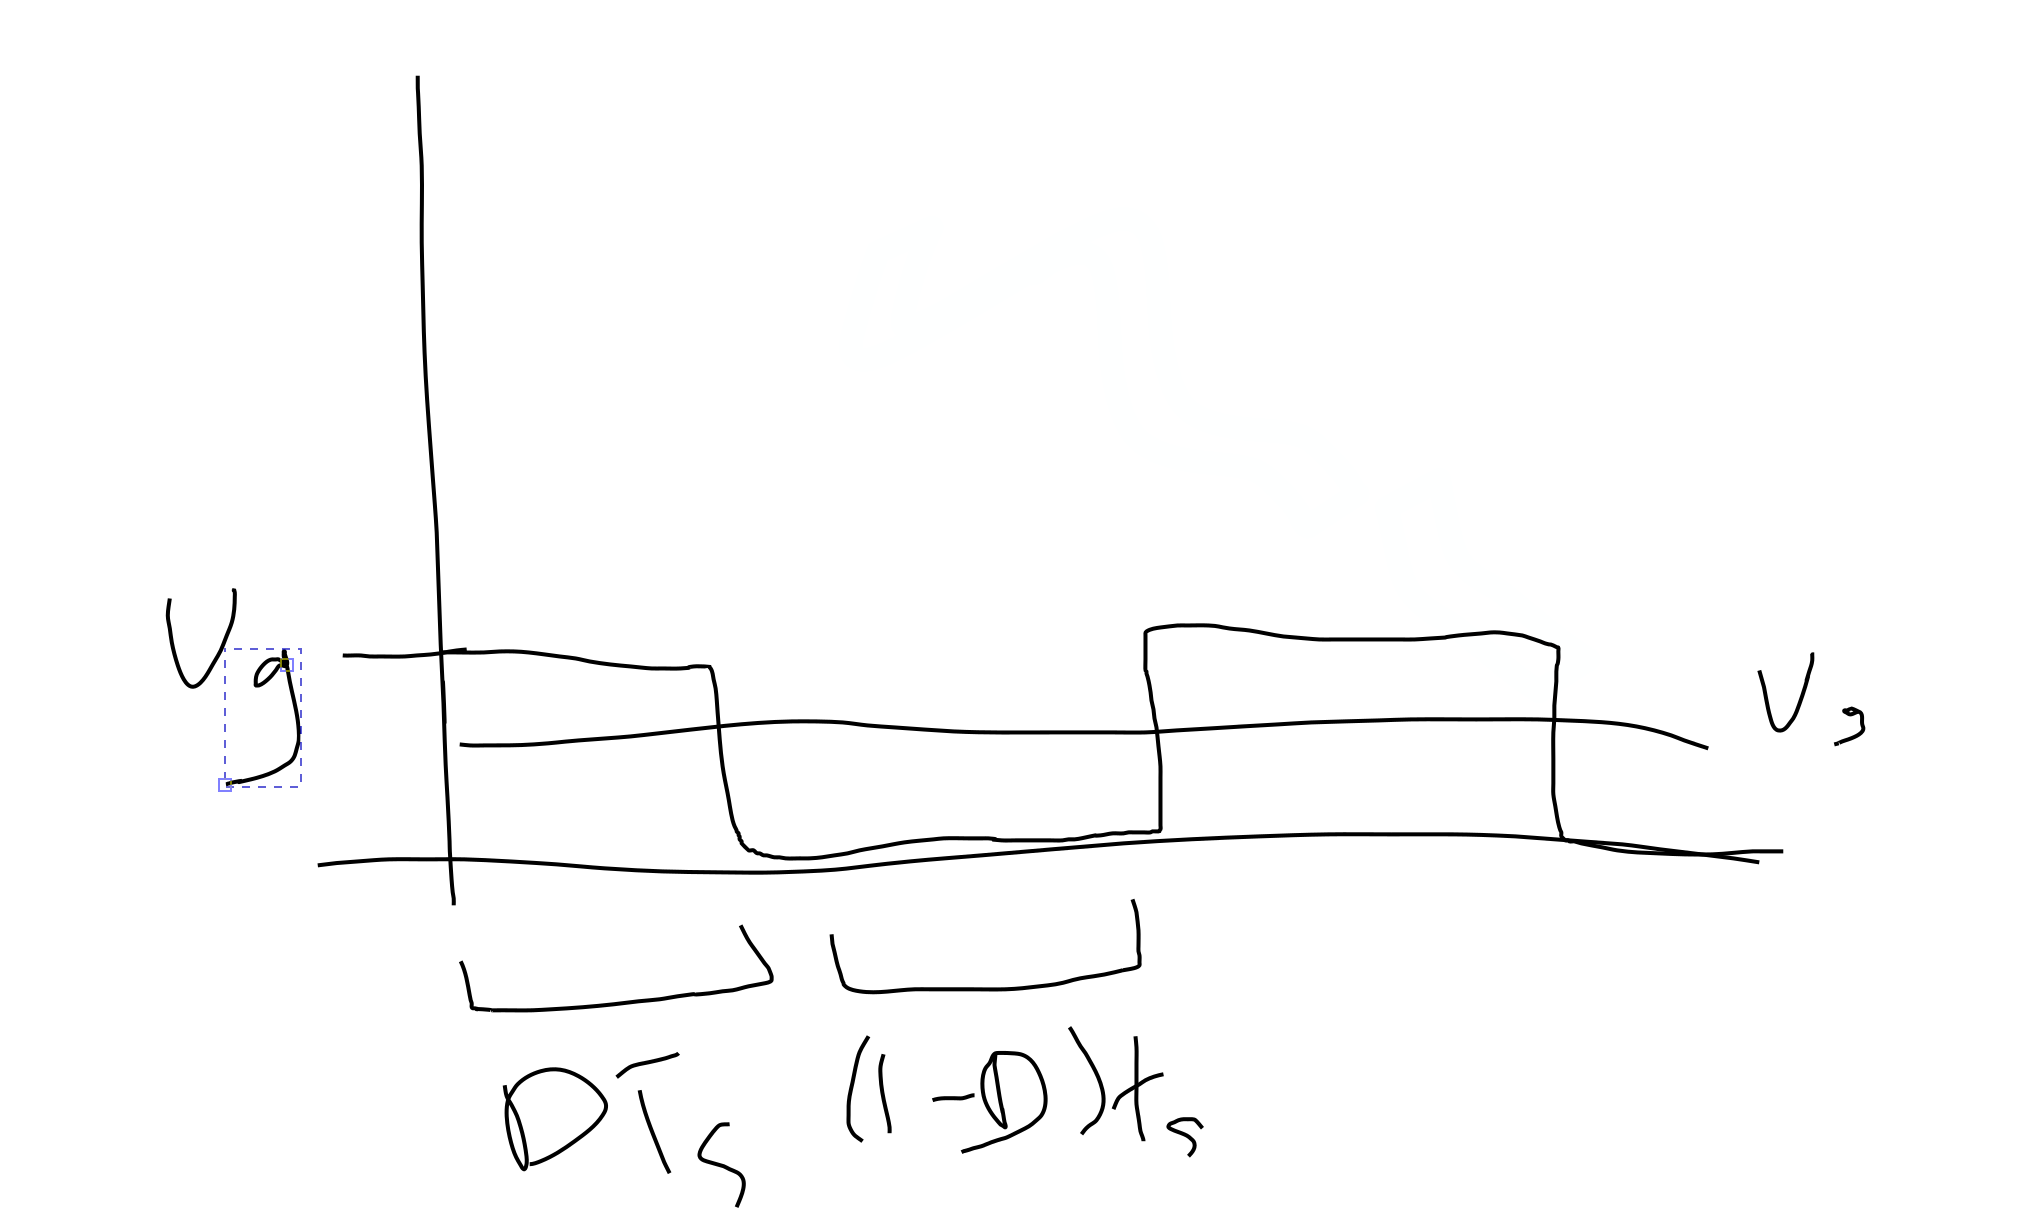
\includegraphics[width=0.8\linewidth]{img/image_2022-09-23-15-26-24.png}
\end{figure}


One problem that we want to characteristic is the ripple voltage, i.e. unwanted harmonics  


\begin{equation}
	v_s(t) = V_s + \sum^{\infty}_{k=1} V_s^k \sin (k \frac{2\pi}{T_s} t)
\end{equation}

The $ V_s $  term is desirable, and the harmonic terms $ V_s^k $ are undesirable.   

\begin{equation}
	V_s^k = \frac{2V_g}{\pi} \sin (k\pi D)
\end{equation}

Basically all Fourier analysis for power electronics will basically always result in an expression with a bunch of terms on one end and then a sin or cos.
$ \frac{1}{k} \frac{2V_g}{\pi} $  is the envelope of the harmonic terms. Note how the envelope decreases with $ k $.


Plotting out the spectrum of signals we get:

\begin{figure}[H]
	\centering
	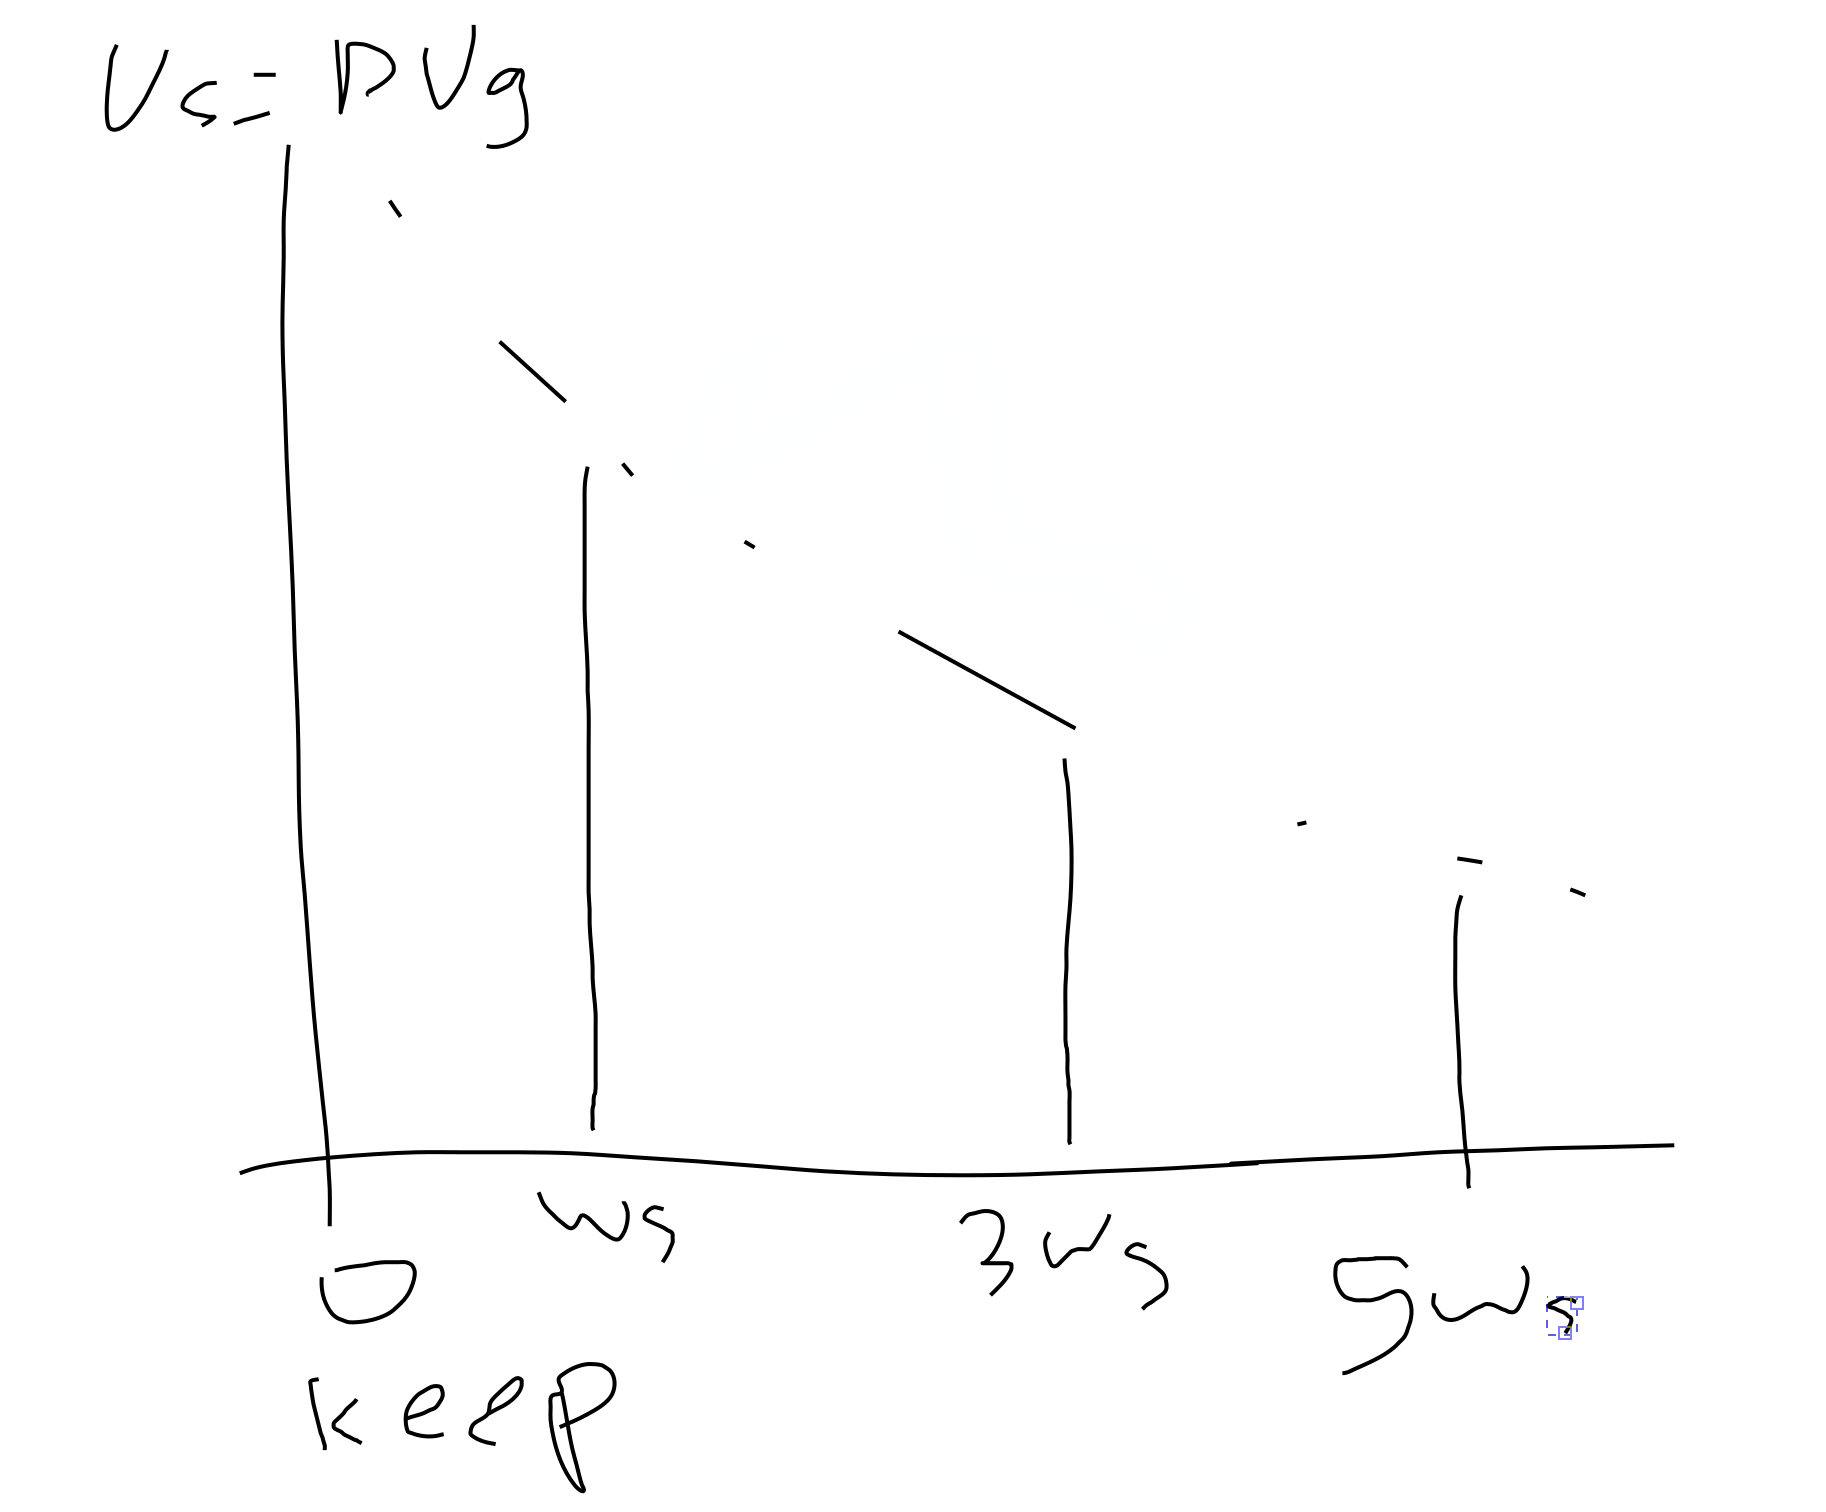
\includegraphics[width=0.8\linewidth]{img/image_2022-09-23-15-29-38.png}
	\caption{Voltage vs frequency. We want to keep the $ \omega=0 $ term and then eliminate the rest with a filter. Note switching frequency $ \omega_s = \frac{2\pi}{T_s} $    }
\end{figure}

\subsubsection{Filtering}

We'll need a ``low pass" filter for dc/dc filtering.

\begin{figure}[H]
	\centering
	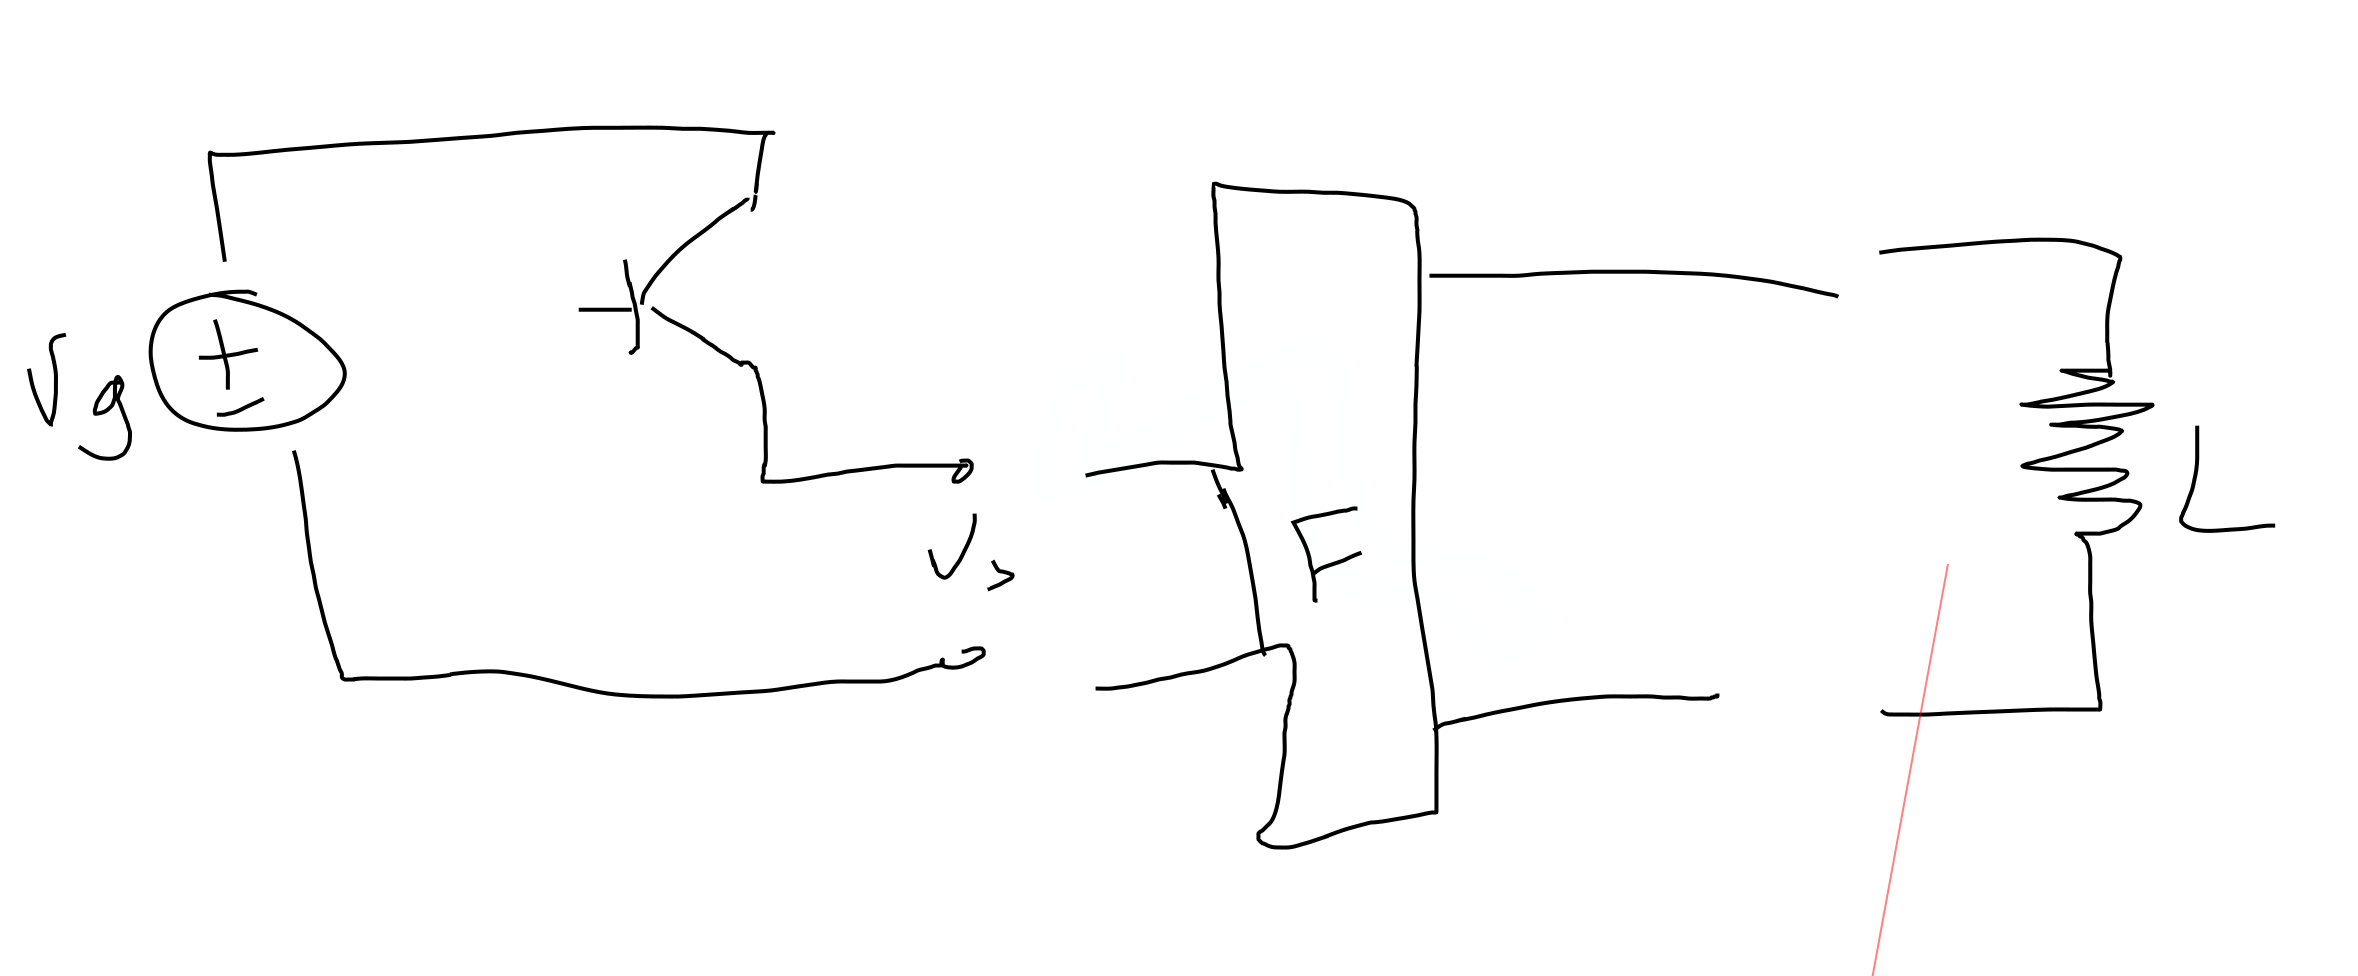
\includegraphics[width=0.8\linewidth]{img/image_2022-09-23-15-33-06.png}
\end{figure}

Choices for filters that may work for this system are the $ RC $, $ LR $ , and $ LC $ filters.
The $ LC $ is most promising because it is second order and it's theoretically lossless because there is no resistor.


We are going to want to maintain continuity of capacitor voltages and inductor currents.
Things work out pretty well while we're on our duty cycle, but once the duty cycle turns off and the switch is opened, $ i \to 0$. 
This is a problem because this will cause us to lose all the energy stored in the inductor everything the switch is opened, which can be a lot given the frequency that these devices operate at.

\begin{equation}
	E = \frac{1}{2} Li^2
\end{equation}

\begin{figure}[H]
	\centering
	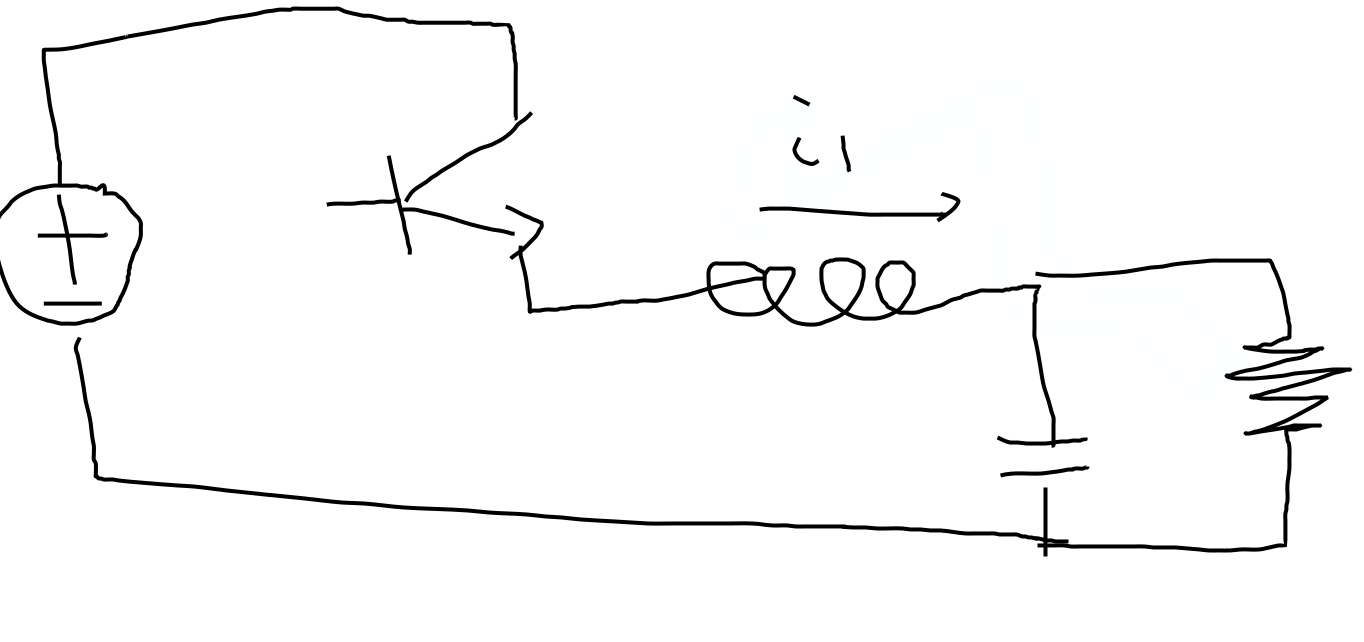
\includegraphics[width=0.8\linewidth]{img/image_2022-09-23-15-39-55.png}
\end{figure}

In order to handle this, we must give the current somewhere to go while off-duty cycle; an energy-recovery diode which ensures that $ i_l $ is continuous and therefore $ E_l $ is lost.
	
\begin{figure}[H]
	\centering
	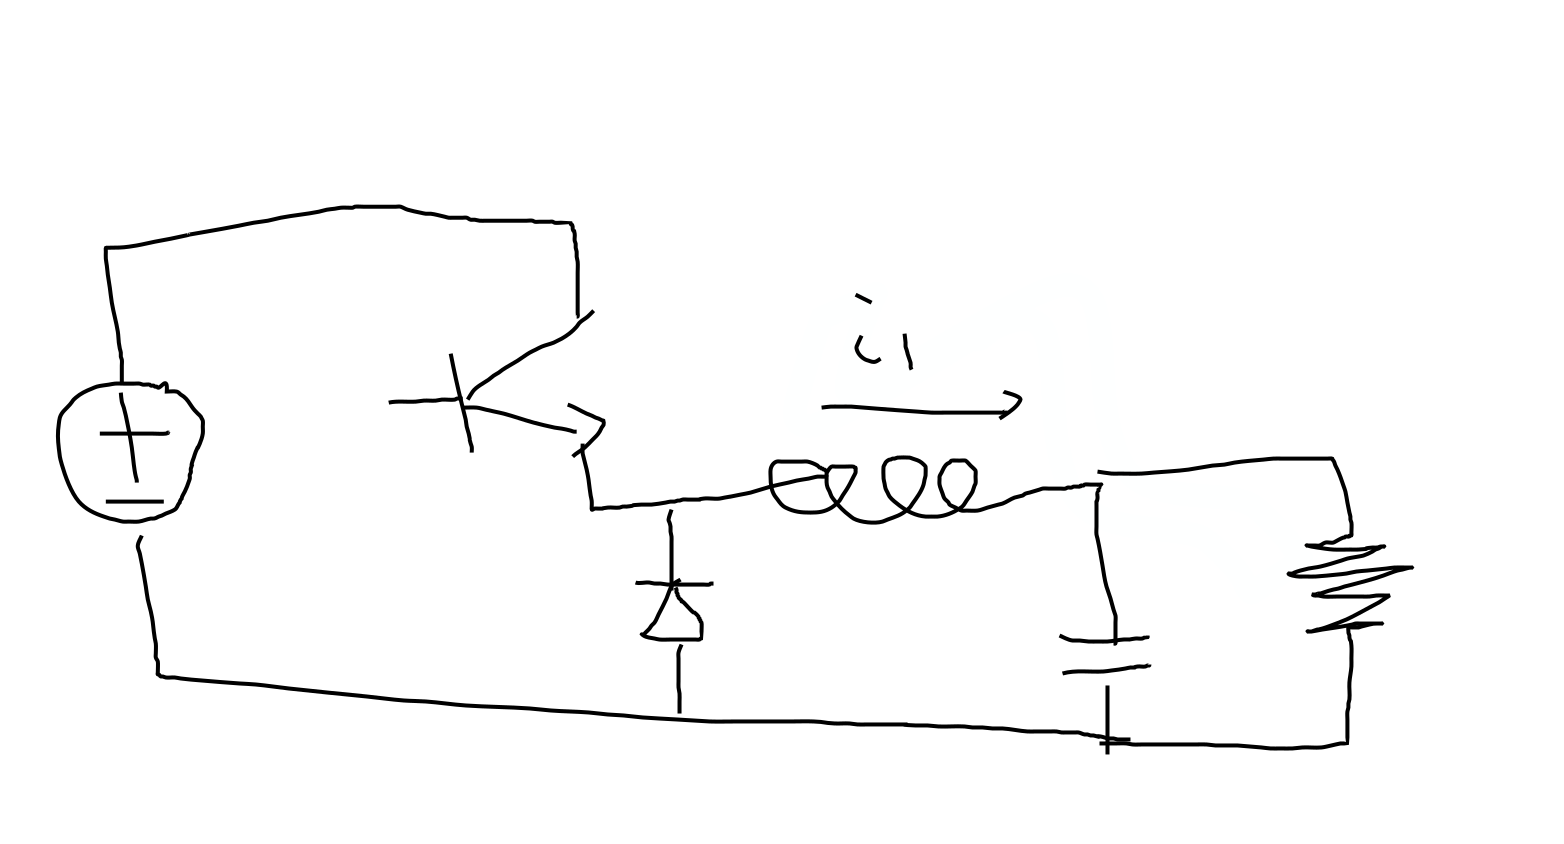
\includegraphics[width=0.8\linewidth]{img/image_2022-09-23-15-40-27.png}
\end{figure}

\begin{blockquote}
	Switching should never yield discontinuity in $ i_l $ or $ v_c $.
\end{blockquote}


Some design considerations:


\begin{enumerate}
	\item Filters all store energy during `on' states and releasing it during `off' states in the magnetic fields of inductors and electric fields of capacitors\marginnote{Capacitors tend to be cheaper so designs are biased to store energy in them instead of inductors}.
	\item Faster switching $ \leftrightarrow  $ less stored energy needed $ \leftrightarrow  $ smaller capacitor and inductor needed
	\begin{itemize}
		\item Switching too fast would cause the system to spend too much time during switching in undesirable high-loss states
	\end{itemize}
\end{enumerate}

Solving these DC-DC converters with Fourier analysis and superposition every time can be a pain, so we'll be looking at other methods next lecture.
Plus, Fourier analysis requires an known $ v(t)$ or $ i(t) $ sources, which is not always the case. 
To motivate this, let's consider the case of an impulse being applied to the system or if the circuit contains diodes.


% \section{Periodic mapping using differential equations}


Periodic mapping using differential equations is a powerful method for solving transients and steady states from solving piecewise linear D.E.s.
This is a whole ton of work so a third method was developed; small-ripple approximation. It only works for steady state\mn{Well, we only use it for steady-state} as it is an approximate solution to the differential equations based on periodic mapping




\subsection{Lecture 9}

A periodic  system is in steady state if

\begin{enumerate}
	\item all input sources are periodic
	\item All states are periodic
	\item switching events are periodic\marginnote{Switching events being literally switching parts of the circuit on/off, i.e. with a transistor}
\end{enumerate}

Consider a simple LR circuit with a $ 33\% $ duty cycle.

\begin{figure}[H]
	\centering
	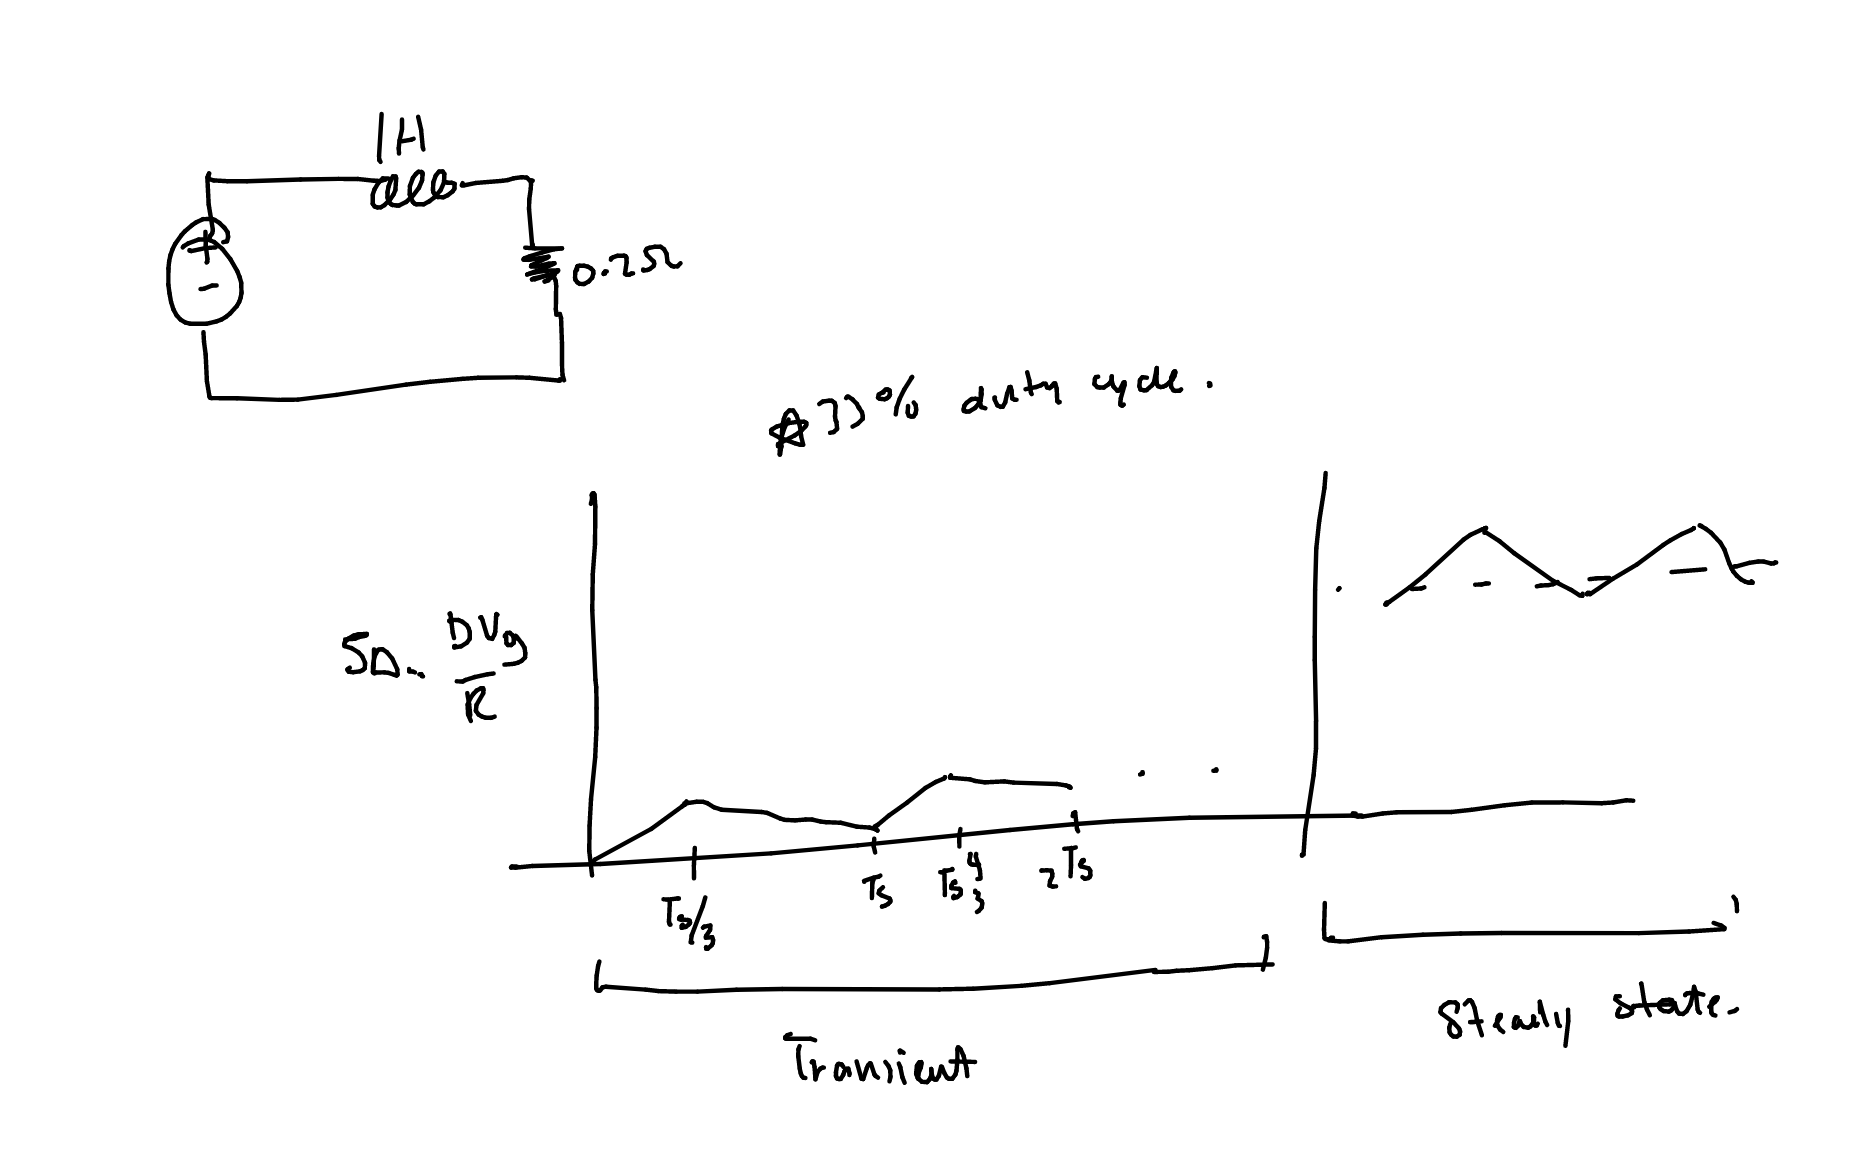
\includegraphics[width=0.8\linewidth]{img/image_2022-09-26-11-35-36.png}
\end{figure}

The system will have an initial transient response before settling down into a steady state.
How can we find this steady state without having to solve for the transients until we get there?


\begin{definition}
\textbf{Steady state}: the net change of state variables over $ T_s $ is zero
\end{definition}


An easier way to find the steady state is to use \textbf{state space averaging}\marginnote{In power electronics this is usually termed small ripple assumption}.

Let's look at a RL circuit and its' steady-state response.

\begin{figure}[H]
	\centering
	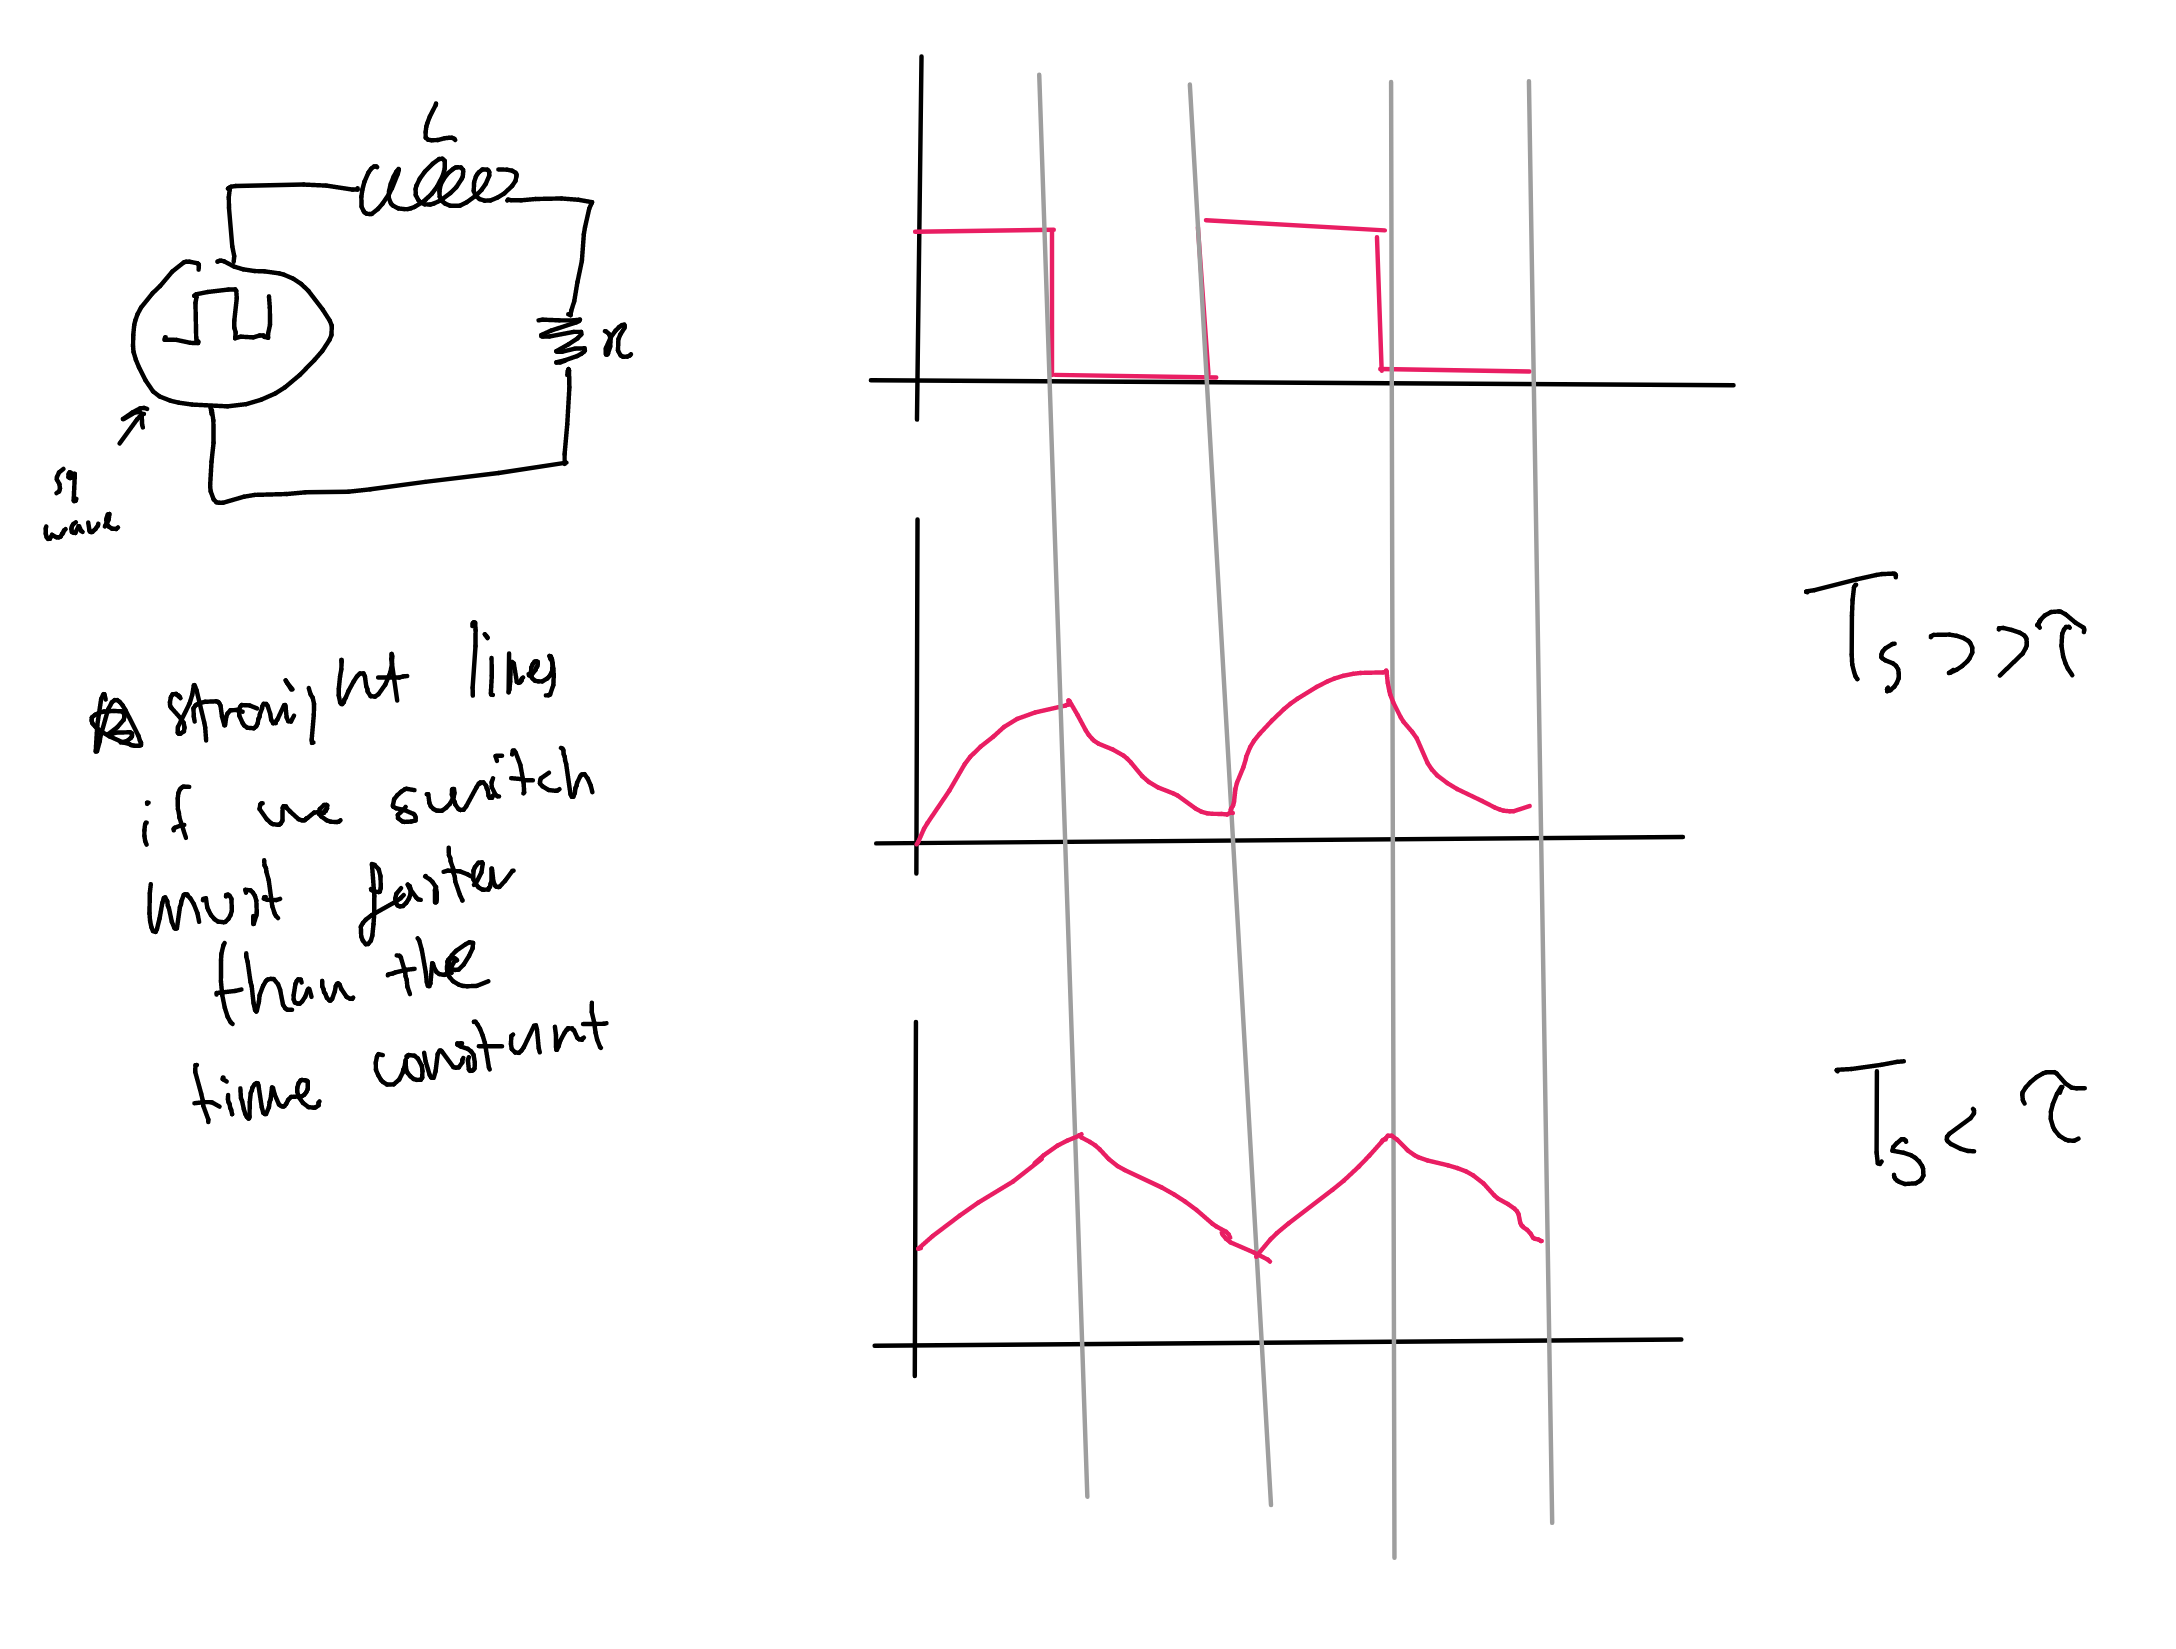
\includegraphics[width=0.8\linewidth]{img/image_2022-09-26-11-35-51.png}
	\caption{Note how the steady-state response becomes a bunch of straight lines if we switch faster than the time constant $ \tau $ }
\end{figure}


\subsubsection{Inductor VoH-Seconds balance}


\begin{equation}
	\begin{split}
		v_l &= L \frac{di_l}{dt}  \\
		i_{l}(t)  &= \frac{1}{L} \int v_l(t) dt  \\
		i_{l}(t+T_s)  &= \frac{1}{L} \int_{t_0}^{t_0 + T_s}  v_l(t) dt + i_l(t_0) \\
		\text{Note: } & 0 = \frac{1}{L} \int_{t_0}^{t_0 + T_s}  v_l(t) dt
	\end{split}
\end{equation}

So, in steady state $ i_l(t_0 + T_s) = i_l(t_0) $ 

\begin{equation}
 0 = \frac{1}{L} \int_{t_0}^{t_0 + T_s}  v_l(t) dt
\end{equation}

This implies that, graphically, the area in the positive part of the $ v(t) $ plot is equal to that of the negative part.


\begin{figure}[H]
	\centering
	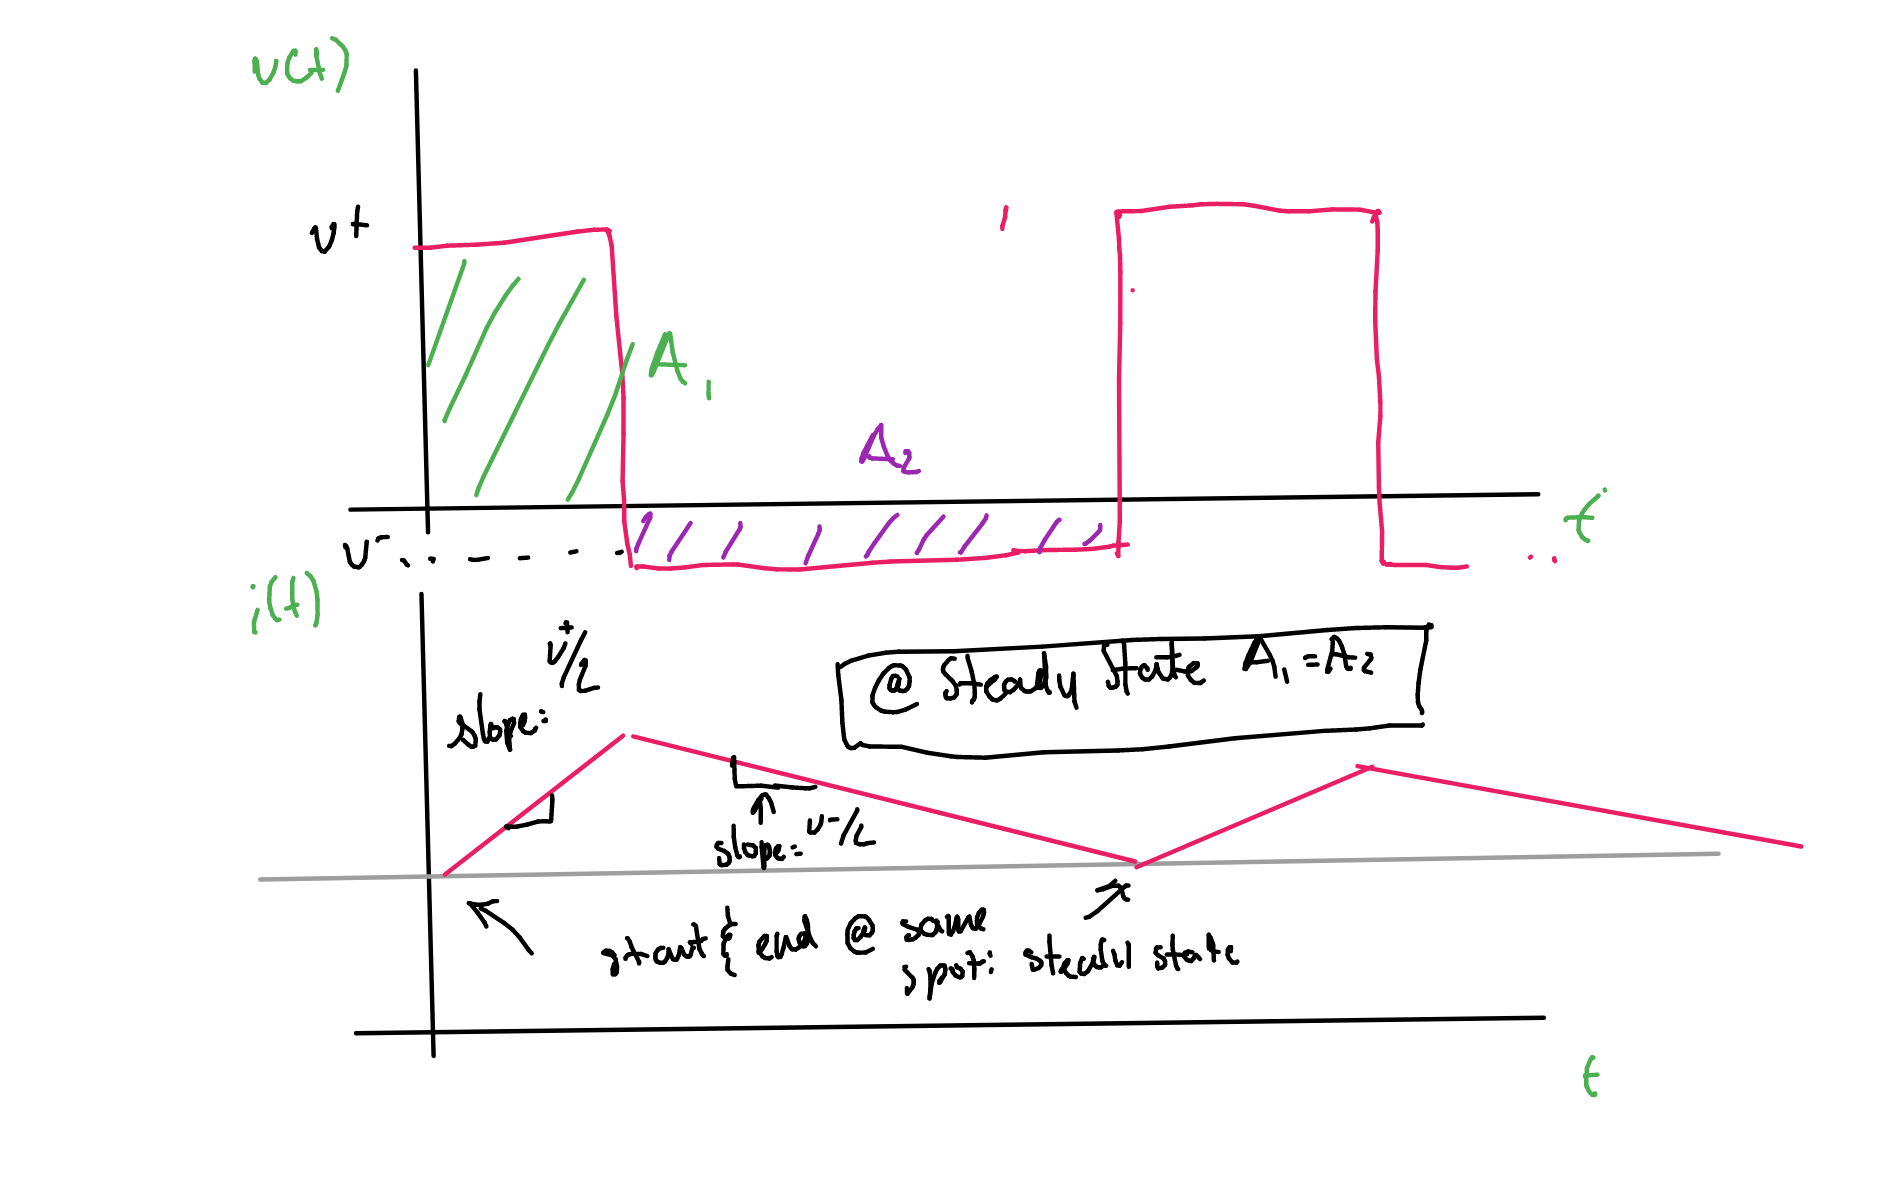
\includegraphics[width=0.8\linewidth]{img/image_2022-09-26-11-44-02.png}
\end{figure}




An analogous relationship can be found for capacitors.

\subsubsection{Capacitor charge balance}
\marginnote{Capacitor balance gives current * time which is charge}


\begin{equation}
	\begin{split}
		i_c(t) &= \frac{d v_c(t)}{dt}\\
		 v_c(t_0+T_s)&= \frac{1}{C} \int_{t_0}^{t_0 + T_s} i_c(t) dt + v_c(t)    \\
	\end{split}
\end{equation}

And at steady state

\begin{equation}
	0 = \frac{1}{C} \int_{t_0}^{t_0 + T_s} i_c(t) dt
\end{equation}


The relationship between the areas above/after the current curve and the voltage response returning to the same spots is the same as that for inductors, just flipped (i.e. voltage areas are equal for inductors but current areas are the same for capacitors).
\begin{figure}[H]
	\centering
	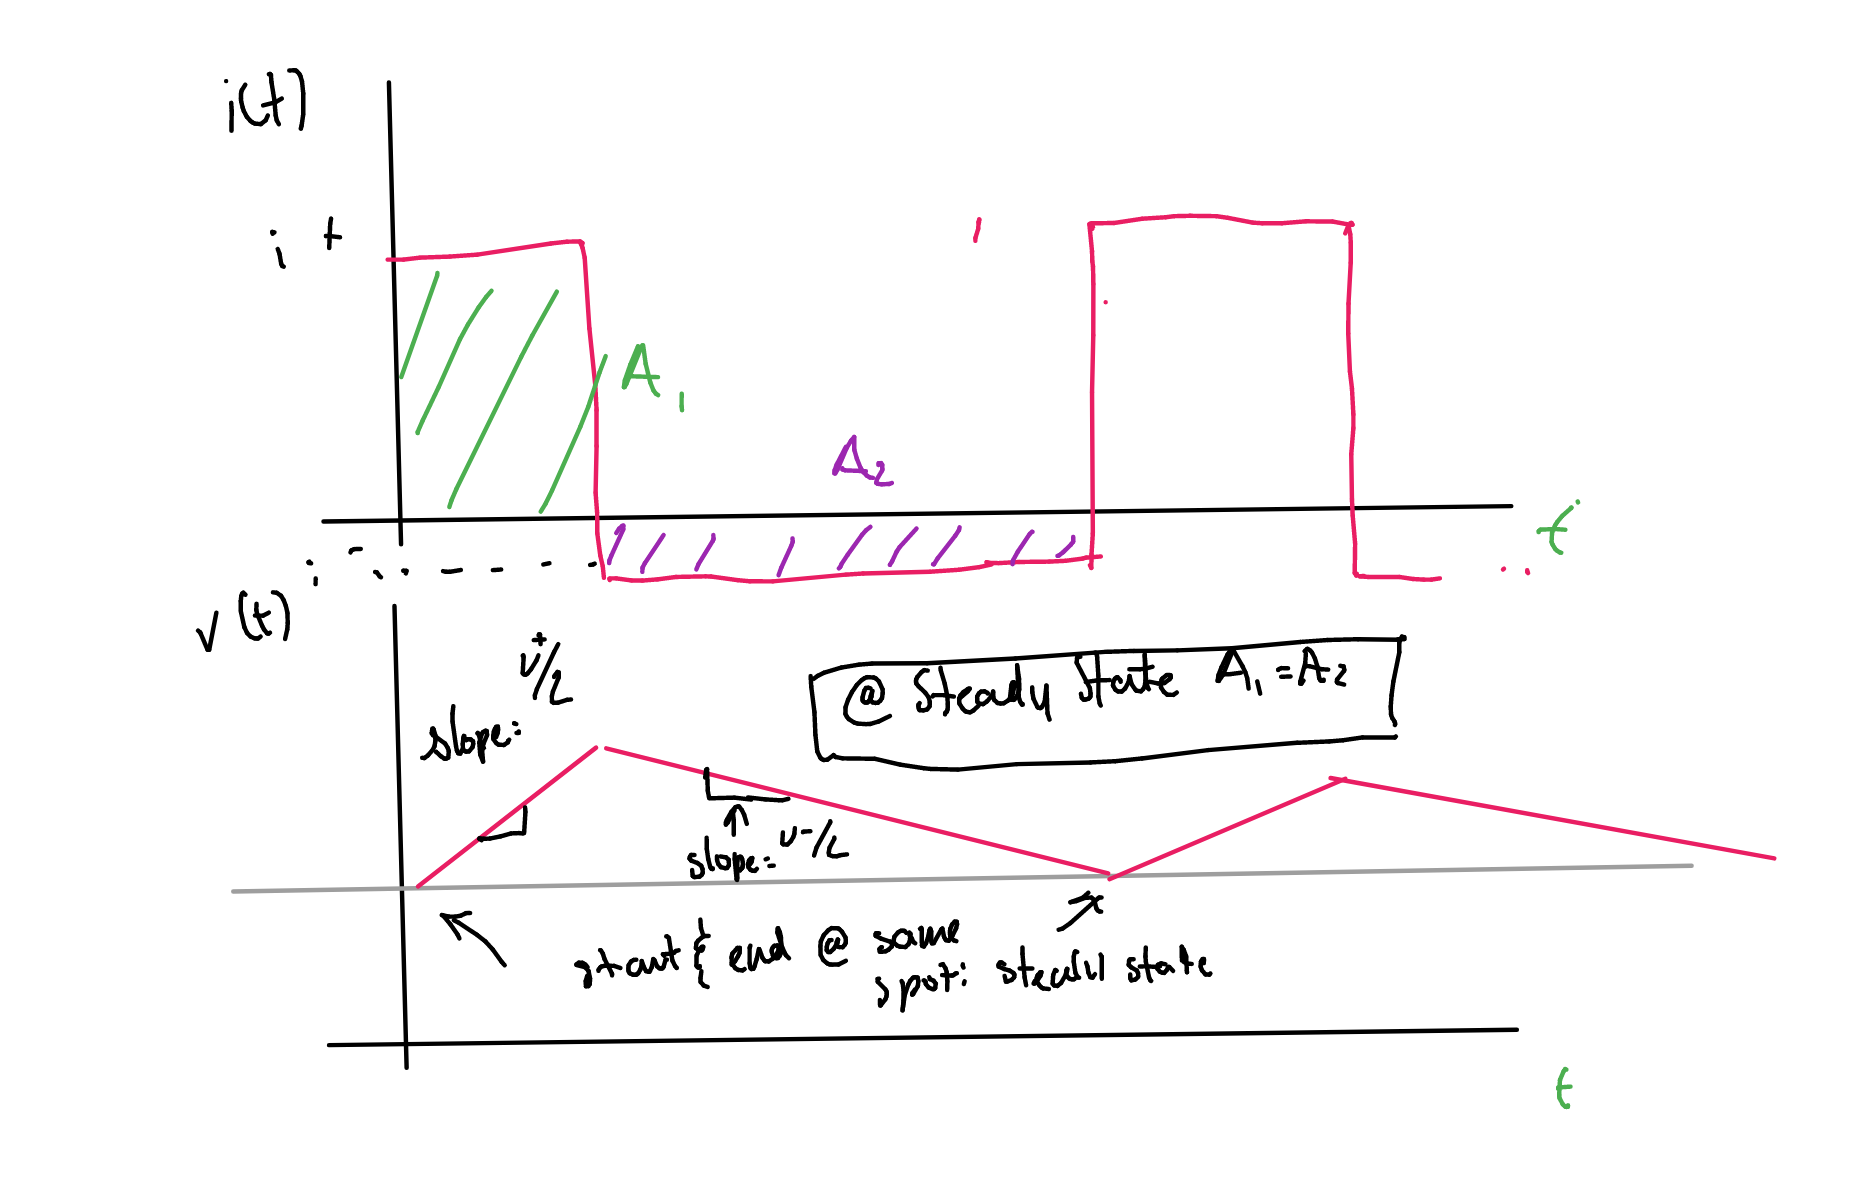
\includegraphics[width=0.8\linewidth]{img/image_2022-09-26-11-51-22.png}
	\caption{This $ A_1 = A_2 $ is the capacitor charge balance}
\end{figure}

\marginnote{$ A_1 $ is adding charge to the capacitor, $ A_2 $ is removing charge}


As an aside it makes our lives easier to define the average current at steady state $ I_R $ so that instead of doing all the math relative to $ 0 $ we can take it to the center of the signal.

What we really want to find is the average $ v_c $ and $ i_l $ 





\subsection{Lecture 10}

\begin{enumerate}
	\item Assume all switches are ideal
	\item Apply small ripple assumption
		\begin{equation}
			\begin{split}
				i_l(t) &\approx I_l  \\
				v_l(t) &\approx V_c 
			\end{split}
		\end{equation}
	\item Sketch waveforms for $ v_l(t) $ for inductors and $ i_c(t) $ for capacitors. These should generally be square in wave shape.
	\item Apply V-s balance and charge balance
	\item Validate ripple sizes and small current assumption
\end{enumerate}



\begin{figure}[H]
	\centering
	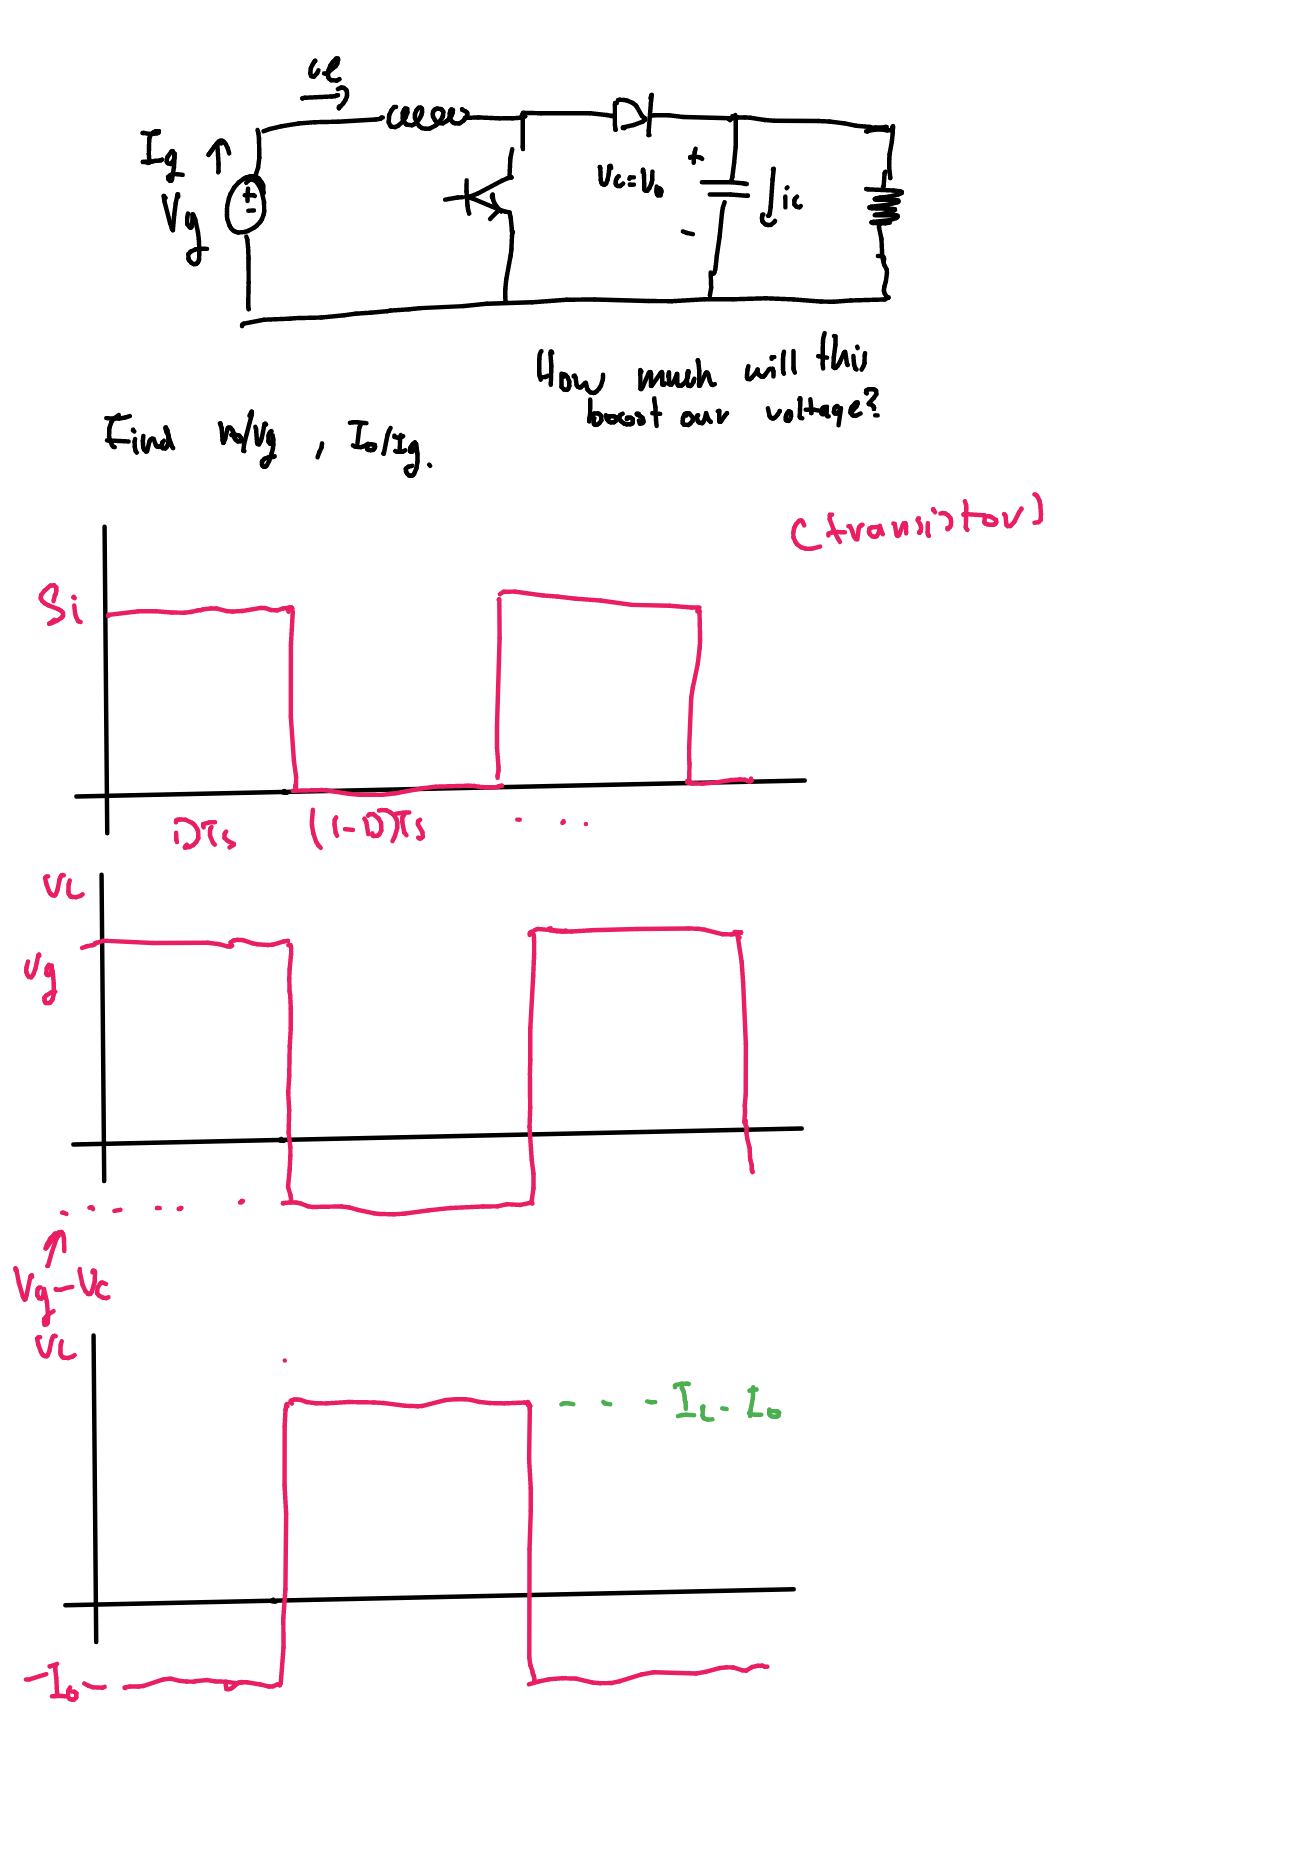
\includegraphics[width=0.8\linewidth]{img/image_2022-09-26-18-29-49.png}
	\caption{Example with a boost converter. Note: 3rd plot should be $i_c$ vs t}
\end{figure}

Applying the $ V-s $ balance:

\begin{equation}
	\begin{split}
		\int_{0}^{T_s} v(t)   & = 0 \qquad \text{or: }  A_1 = A_2\\
		 V_g D  T_s + (V_g - V_c) (1-D) T_s &= 0 \\   
		 V_g &=  V_c(1-D) \\
		 \frac{V_o}{V_g}&= \frac{1}{1-D}  \\
	\end{split}
\end{equation}

What this means is that we can boost $ v $ strongly by modifying the duty cycle $ D $. In theory we can do this infinitely far but in practice after a while physical effects tend to make it really difficult to boost further.


Applying a charge balance:

\marginnote{These integrals can be found by looking at the graphs we drew with the square waves etc and the areas}

\begin{equation}
	\begin{split}
		 \int_{0}^{T_s}  &= i_c(t) dt  \\
										 -I_o (DT_s) + (I_L - I_o) (1-D)T_s &= 0  \\
										 \frac{I_o}{(I_l = I_g)} = 1-D
	\end{split}
\end{equation}

So the output current can similarly be modulated via the duty cycle.


Let's check whether or not if the small ripple assumption is valid.


\begin{figure}[H]
	\centering
	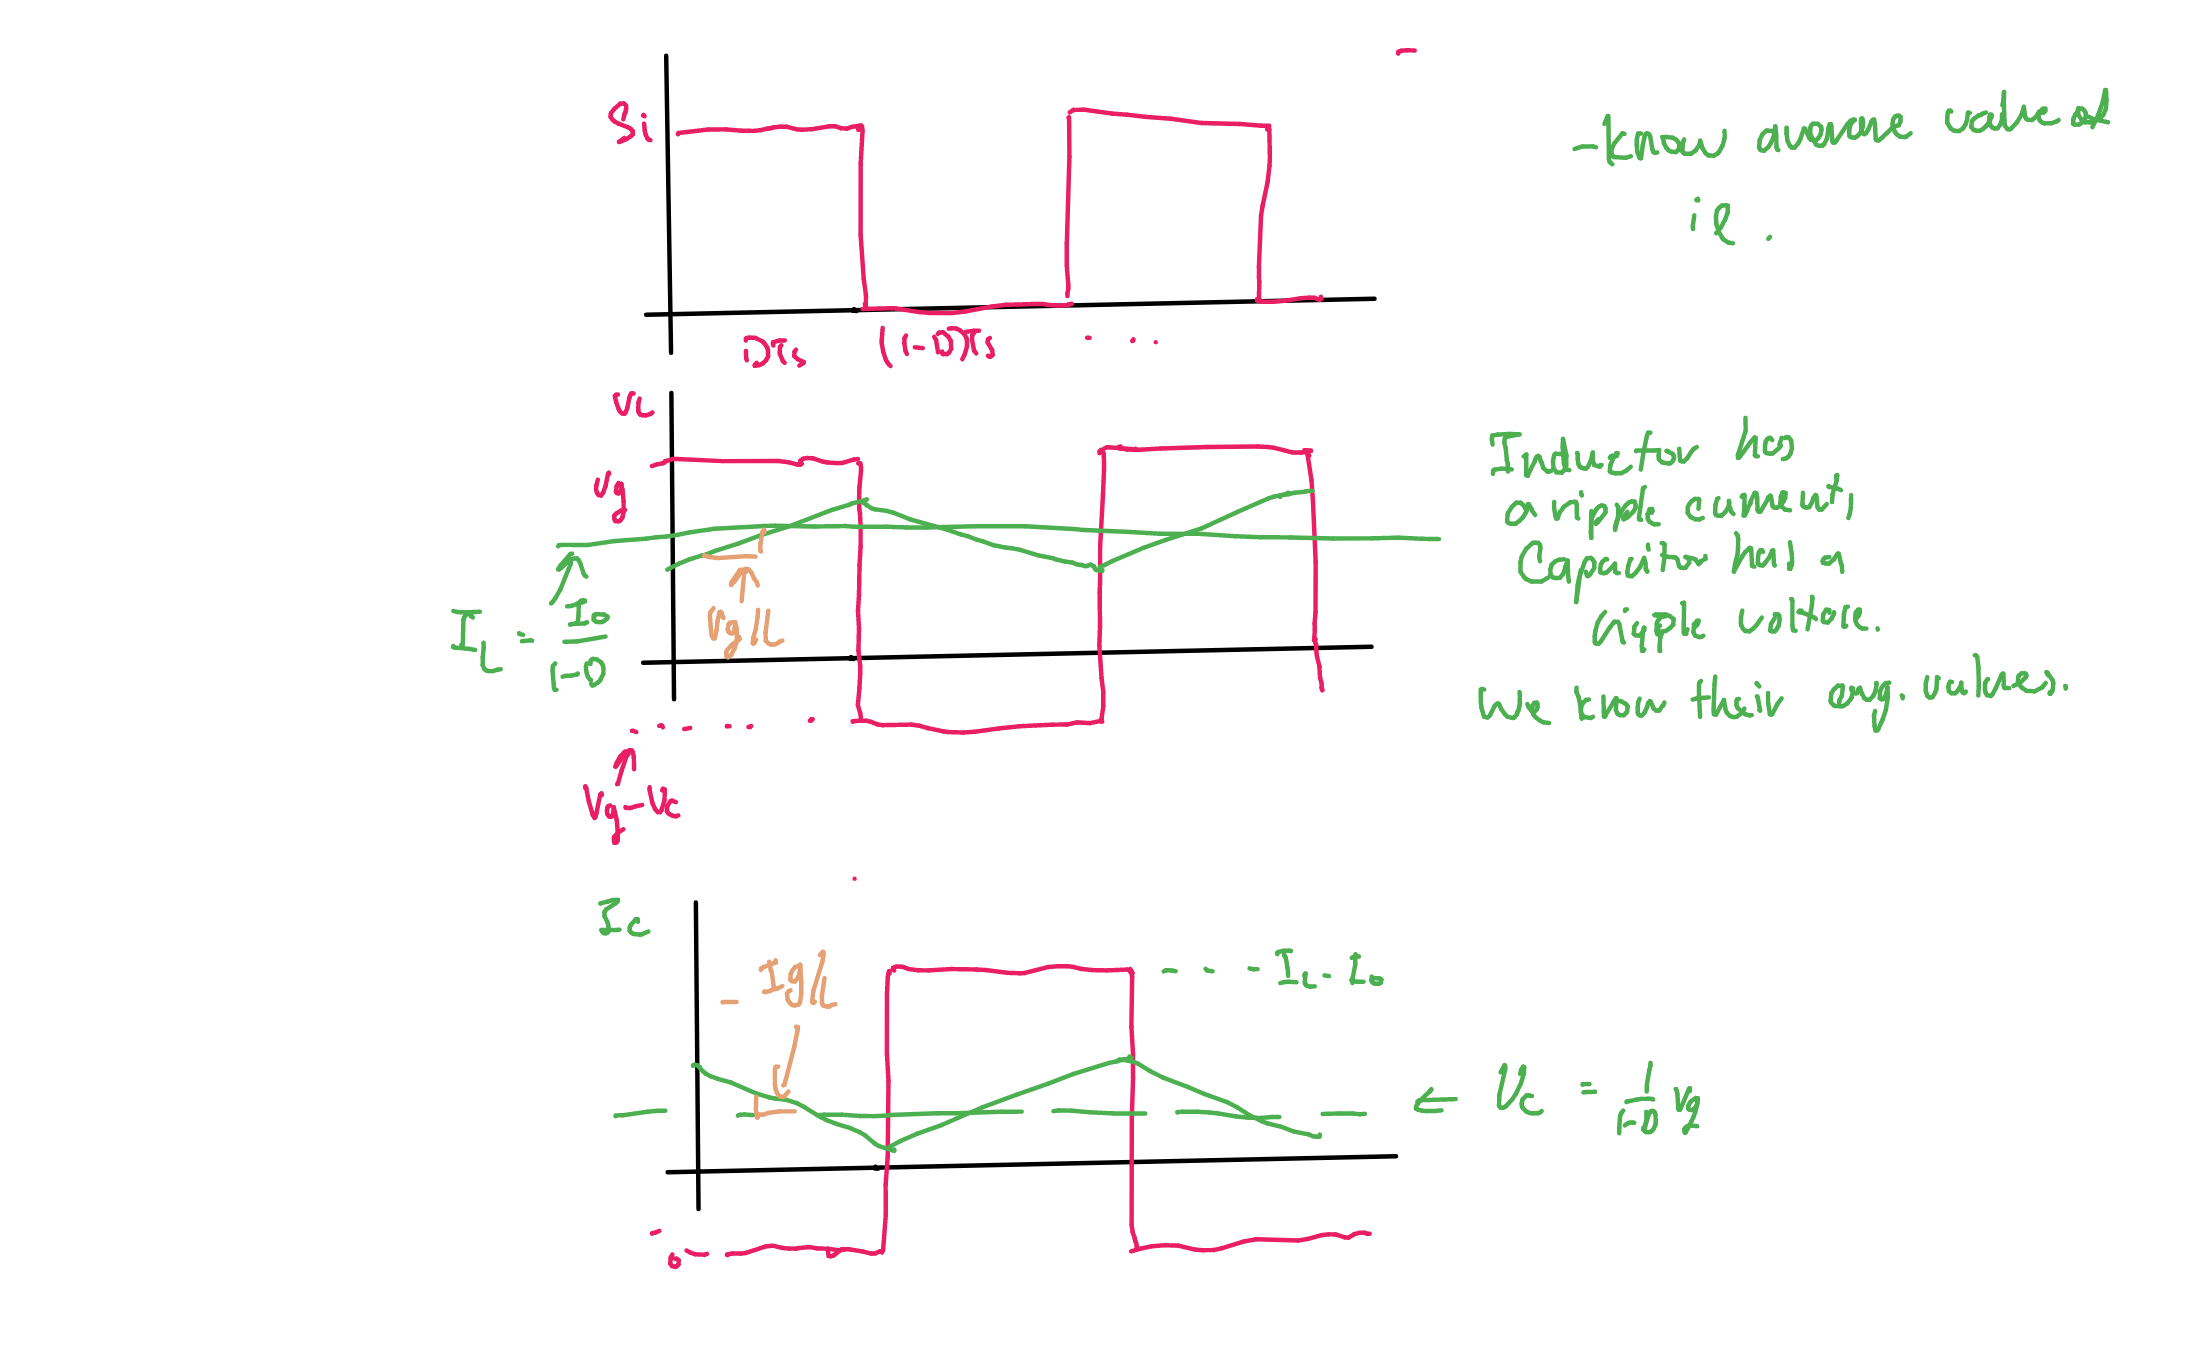
\includegraphics[width=0.8\linewidth]{img/image_2022-09-26-18-45-18.png}
	\caption{Inductor has a ripple current and the capacitor has a ripple voltage. The slope of the roughly saw-shaped waveform is inversely proportional to $ L, C $. So we can pick $ L, C$ such that we get a small enough ripple. }
\end{figure}


So, what defines a `small enough ripple?' 

The amplitude of the ripple is defined from the peak to peak value of the waveform.
\sidenote{The textbook defines it as center to peak, but prof likes peak2peak}


\begin{equation}
	\Delta I_{l p2p} = \frac{1}{L} \int_{0}^{DT_s}  V_g dt = \frac{V_g}{L} D T_{s} 
\end{equation}

\begin{equation}
	\Delta V_{o p2p} = |\frac{1}{C} \int_{0}^{DT_s}  -I_o dt| = \frac{I_o}{C} D T_{s}
\end{equation}

\marginnote{$ V_o = V_c$. Generally we don't care about $ I_{lp2p}  $; it is an internal variable. User only cares about $ V_o $, not $ V_c $ -- they're the same in this case but not necessarily. }


Defining a small ripple is a little more hand-wavy but usually indicates the point at which our approximations start to break down. Generally it means within $ < 30\% $ of the rated current and $ < 30\% $ of the rate voltage. 
But this is highly dependent on the application; a computer PSU would want something a lot cleaner for example.


\subsubsection{Design Process}

\begin{enumerate}
	\item The application will tell the load; $ I_o $, $ V_o $ 
	\item We will have to pick the switch. It'll have to meet the current spec and maybe some thermal design
	\item Look at switch data sheet and then look at the switching frequency that it can run at\mn{Usually smaller switches can run faster than larger ones}
	\item Compute required duty cycle $ D $ for the desired output characteristics $ V_o/V_g $ 
	\item Pick inductor current to achieve the small ripple assumption to get reasonable $ \Delta I_{lp2p}  $. Inductors are more expensive than capacitors so most try to get it to within $ <20\% $ of rated and do the rest using capacitors
	\item Pick $ C $ to meet $ \Delta V_{cp2p}  $  specification
\end{enumerate}



\subsection{Lecture 11}
I slept in and was behind on notes so here are handwritten ones.


\begin{figure}[H]
	\centering
	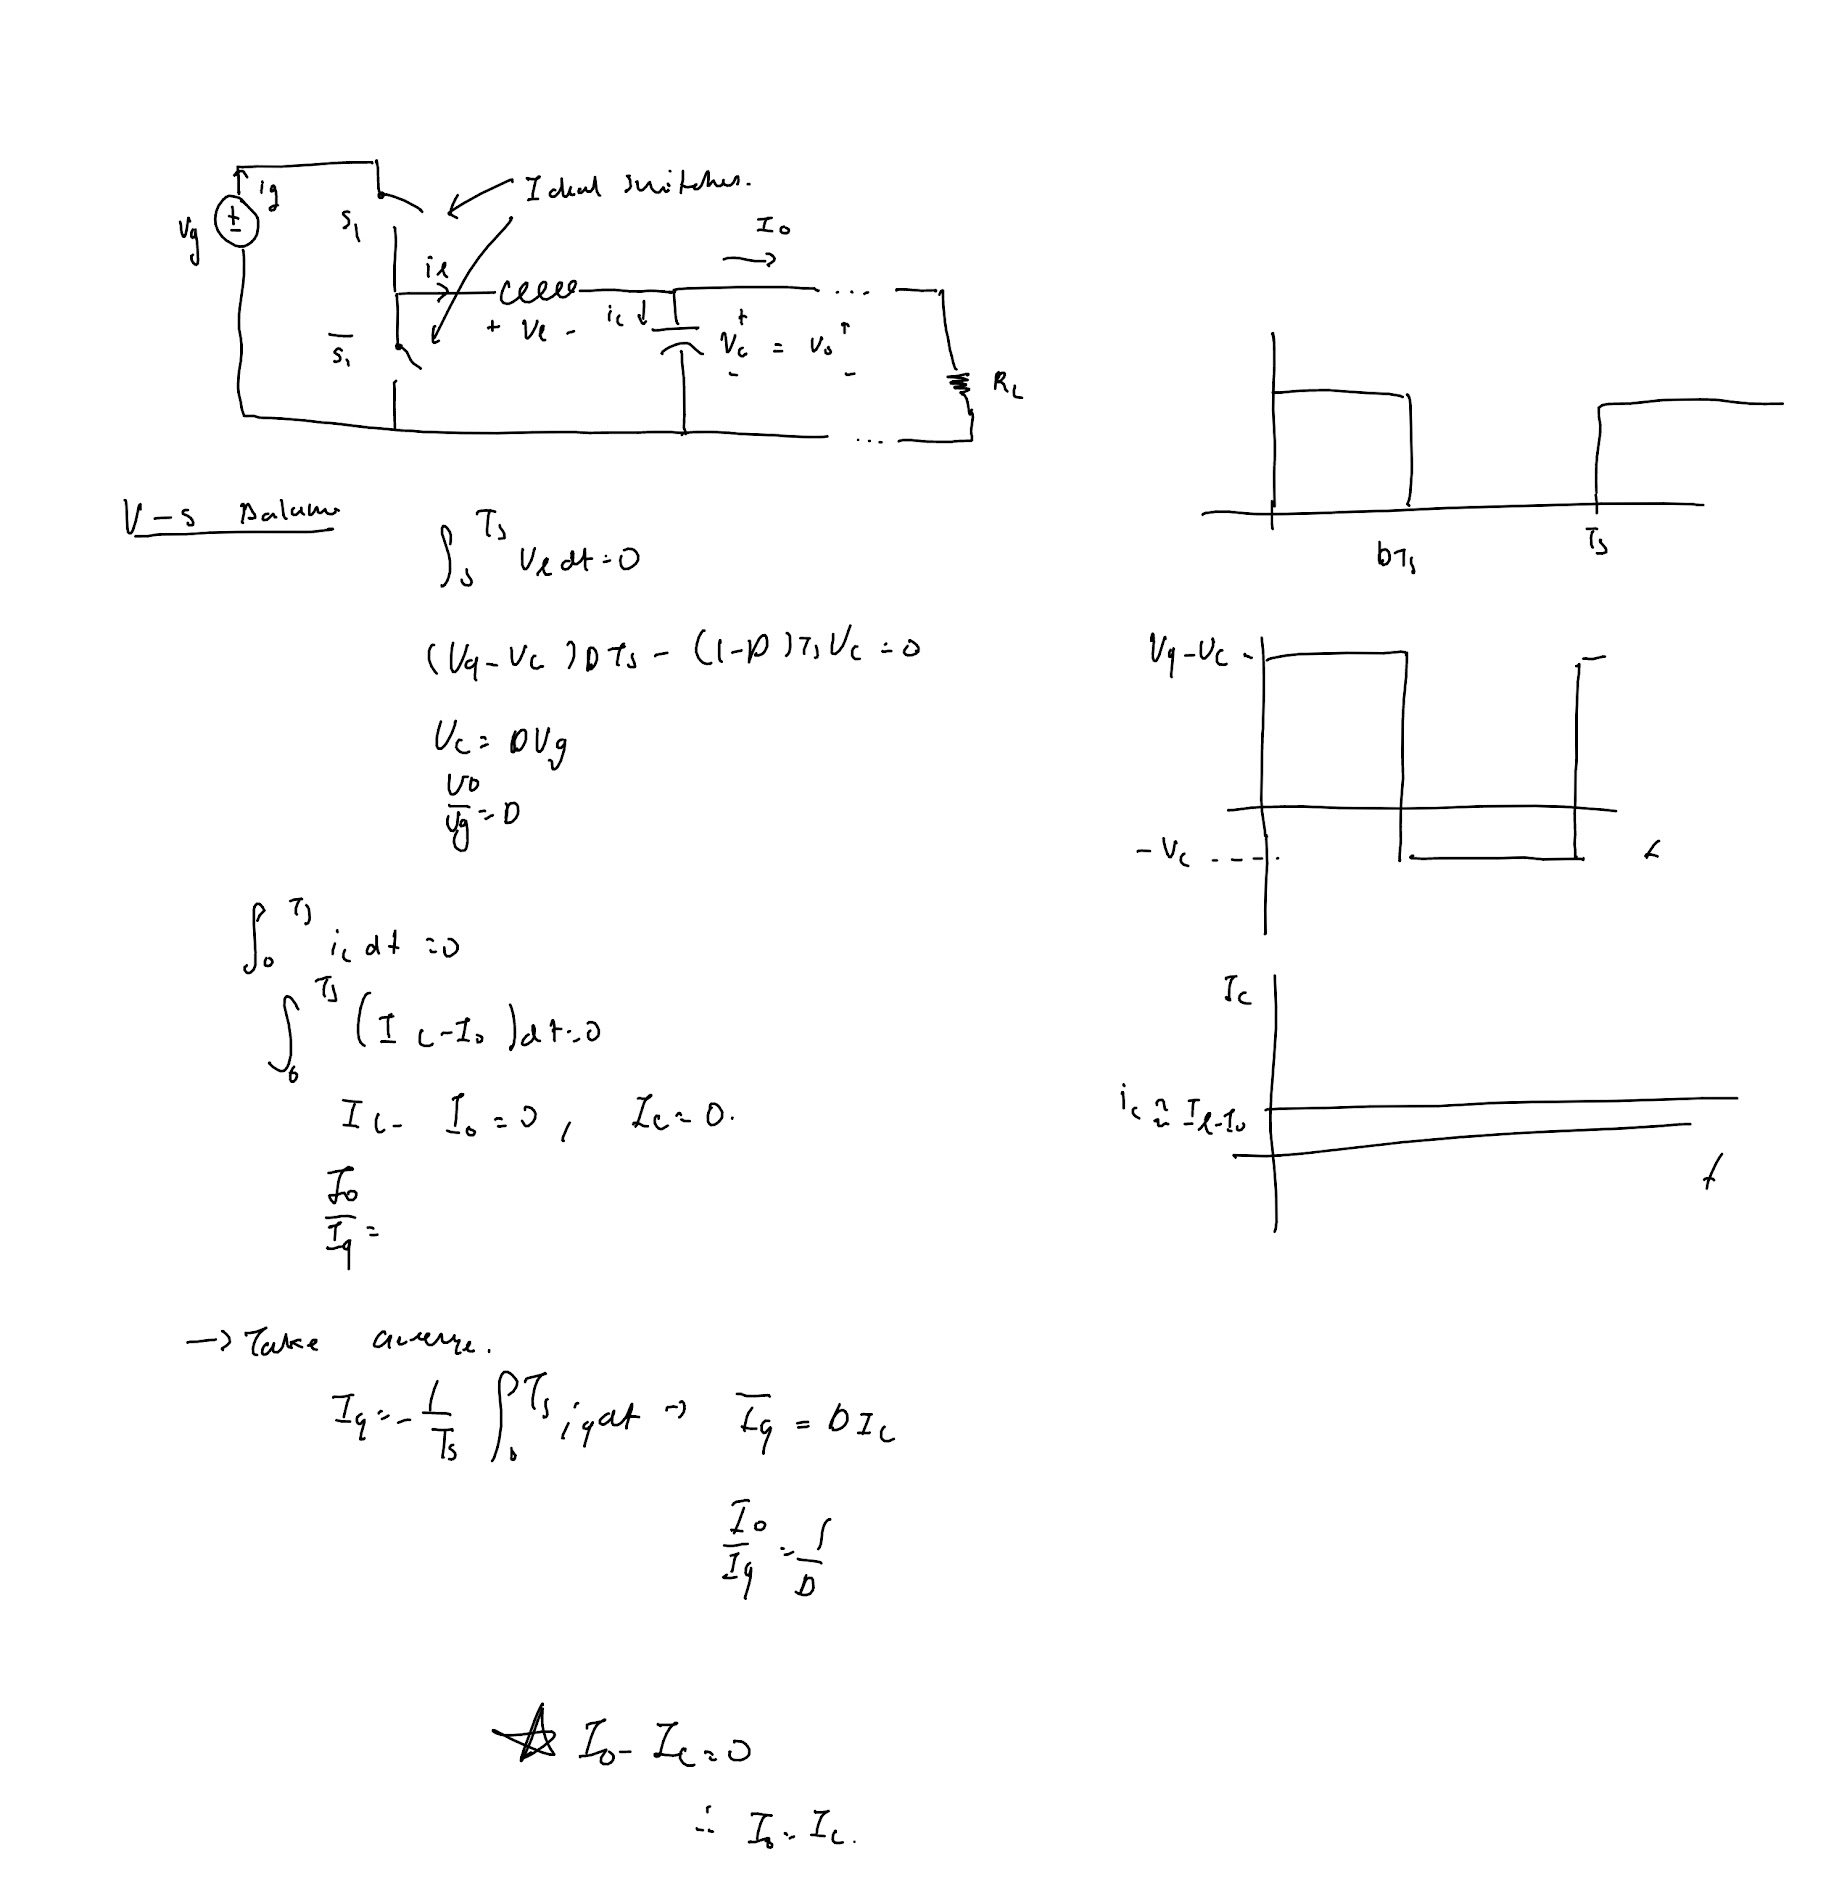
\includegraphics[width=\linewidth]{img/image_2022-09-29-11-58-31.png}
\end{figure}

\begin{fullpage}

\begin{figure}[H]
	\centering
	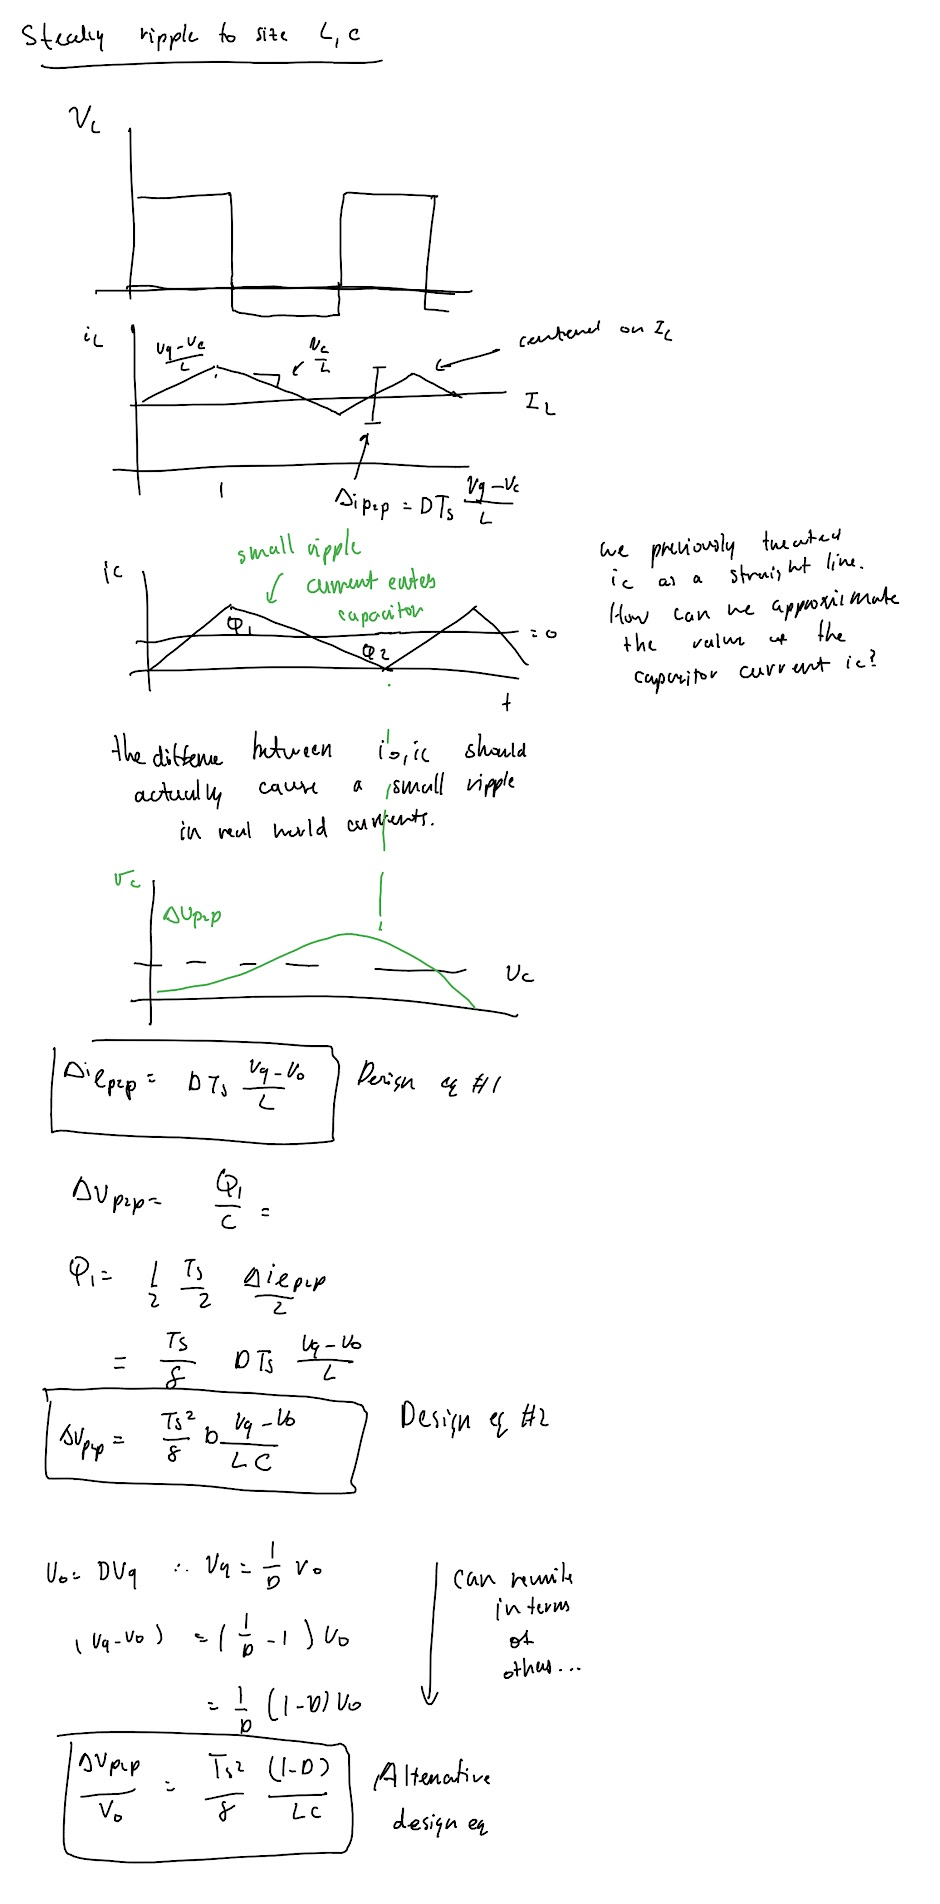
\includegraphics[width=0.6\linewidth]{img/image_2022-09-29-11-58-49.png}
\end{figure}

\end{fullpage}


\subsection{Lecture 12}

\end{document}

% 349 END
